\documentclass[12pt]{report} % Default font size is 12pt, it can be changed here

\usepackage{geometry} % Required to change the page size to A4
\geometry{a4paper} % Set the page size to be A4 as opposed to the default US Letter
\geometry{left=2cm,right=2cm,top=2.5cm,bottom=2.5cm}
\usepackage{cite}

\usepackage{color}
\usepackage{csvsimple}
\usepackage{xcolor}
\usepackage{numprint}

\usepackage{datetime}%%display time
\newdateformat{MY}{\monthname[\THEMONTH], \THEYEAR}


\usepackage{graphicx} % Required for including pictures
\usepackage{subfig}

\usepackage{tikz}%%flow chart package
\usetikzlibrary{shapes.geometric, arrows}
\tikzstyle{startstop} = [rectangle, rounded corners, minimum width=3cm, minimum height=1cm,text centered, draw=black, fill=red!30] %%flow chart style
\tikzstyle{io} = [trapezium, trapezium left angle=70, trapezium right angle=110, minimum width=3cm, minimum height=1cm, text centered, draw=black, fill=blue!30]
\tikzstyle{process} = [rectangle, minimum width=3cm, minimum height=1cm, text centered,text width=4.5cm ,draw=black, fill=yellow!30]
\tikzstyle{decision} = [diamond, minimum width=3cm, minimum height=1cm, text centered, draw=black, fill=green!30]
\tikzstyle{arrow} = [thick,->,>=stealth]%%arrow style
\tikzstyle{line} = [draw, thick, -latex']

\usepackage{etoolbox}
\patchcmd{\abstract}{\titlepage}{\titlepage% Insert ToC-writing after starting a titlepage
  \addcontentsline{toc}{chapter}{Abstract}}{}{}
\setcounter{secnumdepth}{3}
\setcounter{tocdepth}{3}

\usepackage[nottoc]{tocbibind}
\usepackage{float} % Allows putting an [H] in \begin{figure} to specify the exact location of the figure
\usepackage{wrapfig} % Allows in-line images such as the example fish picture
\usepackage{titling}

\usepackage{booktabs}
\usepackage{array}
\usepackage{lipsum} % Used for inserting dummy 'Lorem ipsum' text into the template
\usepackage{amsmath}
\usepackage{framed}
\usepackage{amssymb}
\usepackage{authblk}


\usepackage{enumerate}
\usepackage{setspace}
\linespread{1.5} % Line spacing
\setlength\parindent{0pt} % Uncomment to remove all indentation from paragraphs

\graphicspath{{Pictures/}} % Specifies the directory where pictures are stored
\usepackage{blindtext}
\newcommand{\norm}[1]{\left\lVert #1 \right\rVert}

\begin{document}
\begin{center}

\begin{large}
WORCESTER POLYTECHNIC INSTITUTE\\
\end{large}
\begin{Large}
\textbf{Kernel Coherence Encoder}

\end{Large}

by\\
Fangzheng Sun\\
A thesis\\
Submitted to the Faculty\\
of the\\
WORCESTER POLYTECHNIC INSTITUTE\\
in partial fulfillment of the requirements for the\\
Degree of Master of Science\\
in\\
Data Science\\
\vspace{15 bp}
\begin{large}April 2018\\
\end{large}
\end{center}
\vspace{2 in}

\noindent\begin{tabular}{ll}
APPROVED:\\[1ex]
Professor Randy C. Paffenroth, Adviser:\\[5ex]
\makebox[3.5in]{\hrulefill} \\
Professor Jian Zou, Reader:\\[5ex]
\makebox[3.5in]{\hrulefill}\\
\end{tabular}

\clearpage


\tableofcontents
\clearpage

\begin{center}
	\addcontentsline{toc}{chapter}{Abstract}
	WORCESTER POLYTECHNIC INSTITUTE\\
	\vspace{1 in}
	\begin{Large}
		\emph{Abstract}\\
	\end{Large}
	\vspace{30 bp}
	\begin{small}
		Data Science\\
	\end{small}
	\vspace{15 bp}
	\begin{small}
		Master of Science\\
	\end{small}
	\vspace{15 bp}
	\begin{small}
		by Fangzheng Sun\\
	\end{small}
\end{center}
In this thesis, we introduce a novel model based on the idea of autoencoders. Different from a classic autoencoder reconstructing its own inputs through a neural network, our model learns an idea from Kernel Canonical Correlation Analysis (KCCA) and reconstructs input data from another data set, where these two data sets should have some correlation. Our model extends traditional KCCA in a way that the non-linearity of the data is learned through optimizing a kernel function by a neural network. In one of the novel parts of this thesis, we do not optimize our kernel based upon some prediction error metric, as is classical in autoencoders. Rather, we optimize our kernel to maximize the ``coherence'' of the underlying low-dimensional hidden layers. This idea makes our method faithful to the classic interpretation of linear Canonical Correlation Analysis (CCA). 
As far we are aware, our method, which we call a \textit{Kernel Coherence Encoder (KCE)},  is the only extent approach that uses the flexibility of a neural network, while maintaining the theoretical properties of classic KCCA. In another one of the novelties of our approach, we leverage a modified version of classic coherence which is far more stable in the presence of high-dimensional data to solve computational and robustness issues in the implementation of a coherence based deep learning KCCA.

\clearpage

\chapter{Introduction}
In the recent years, the concept of deep learning is becoming a hot topic for divergent industries as well as multiple fields of study\cite{AUKM,TF,PR,DLRG}. Deep learning is a subfield of machine learning. There are many sub-categories of deep learning. Herein, we focus on artificial neural network (ANN)\cite{NN,NN2} and autoencoders\cite{AE,AE2,AE3} that allow us to discover non-linear low-dimensional manifold. Such methods are frequently used for unsupervised learning and for producing low-dimensional representations of data. Typically, an autoencoder consists two parts, an encoding phase (encoder) \(E(\cdot)\) and an decoding phase (decoder) \(D(\cdot)\). The encoder \(E(\cdot)\) takes the input data and maps it to a low-dimensional representation. The decoder \(D(\cdot)\) then takes this low-dimensional representation and attempt to reconstruct the original high-dimensional data.\\
Note, such an autoencoder is closely related to Principal Component Analysis (PCA)\cite{PCA,PCA2,STAT,KPCA}. In fact, an autoencoder is identical to PCA when each layer is assumed to be linear and the reconstruction cost function is Euclidean distance. In particular, many people are attracted by the nonlinear aspect of autoencoders, which makes it more powerful than a typical PCA, and effective in solving more real-life problems.\\
We create three novel models to leverage the full power of the autoencoders. Our first model, Non-Coherence Encoder (NCE), is built upon both linear and non-linear autoencoders. Then we move on to CCA\cite{CCA,ECCA} and KCCA\cite{KCCA}, merging their strengths with the autoencoder approach in another two proposed models, Coherence Encoder (CE) and Kernel Coherence Encoder (KCE) respectively. When we test their performance by the MNIST\cite{MNIST} digit image data set, we find that with these CCA tricks, especially KCCA, the reconstruction images tend to be closer to original images. \\

\section{Motivation}
Let us begin the story of our research with some interesting questions one may have: at the age of 20, can you predict your looking at the age of 40? Or, when you look at a 40-year-old person, can you imagine what he or she looks like at the age of 20? A human brain, based on visual observations, learns and finds a ``mapping" between a 20-year-old face and a 40-year-old face. Consequently, people might be able to give reasonable answers to the above questions.\\
We want our models to mimic this learning process of a human brain while maintaining its own trick to extract the ``correlation" between data sets. Our purpose is to reconstruct two ``potentially correlated datasets" from one to another. An autoencoder focuses on one input data set. Given two correlated data sets, we introduce CCA and even further its kernel version KCCA to dig out the correlation between them. \\
The idea of applying kernel methods to autoencoders also comes from Yan Pei's work \textit{Auto-encoder Using Kernel Methods}\cite{AUKM}. In his model, he replaces the encoder part of an autoencoder with Kernel PCA (KPCA)\cite{KPCA} and the decoder with kernel-based linear regression. It is a model that is designed to work similarly as an autoencoder, but remains faithful to the ``kernel trick''. The ``kernel trick'', which will be discussed in detail in the next chapter, is a classic technique for non-linearly projecting features to a high-dimensional space, gaining the benefit of complex non-linear features, without incurring the cost of working directly in a high-dimensional space. Although it is reasonable, and perhaps even obvious, to try to connect the kernel trick and deep learning, it is notable that, as far as we are aware, the current methods such as \cite{AUKM}, do not leverage the full power of autoencoders.\\

\section{Contribution}
NCE is built upon a similar structure with two independent autoencoders containing both linear and nonlinear layers. Each ``autoencoder'' maps one data set to the other. Nevertheless, the experimental results with MNIST digit image data indicate its deficiency. \\
We gain the initial vision of CCA through \textit{Empirical canonical correlation analysis in subspaces}\cite{ECCA}. This paper provides detailed explanations of CCA, including the calculations for canonical variables of data pairs. Meanwhile, we are inspired by the authors' idea to maximize their coherence through CCA. CCA and PCA differ that PCA attempts to reconstruct a set of data from itself, while CCA has two data sets, and it tries to reconstruct one data set from the other. It is this added complexity of having two data sets that make our proposed model non-trivial to develop.\\
However, in most real-life problems, the correlations of the data sets are not necessarily linear, thus calculating their linear coherence may not be the best solution to dig their correlations. We take a further step to its kernel version, KCCA. With the help of deep learning, we initialized a kernel function with some hyperparameters and train the kernel function to maximize the coherence of two data sets in the RKHS. Then we extract the canonical variables for data reconstruction.\\
In another two models, CE and KCE, we take advantage of CCA and KCCA respectively. While CE rests upon the combination of linear CCA and autoencoders, in KCE we extend the traditional CCA from linear to non-linear by kernel methods and increase the performance of CCA in a similar way by leveraging the non-linear capabilities of autoencoders.\\
At a high level, our KCE method proceeds in two phases, the \textit{encoder} and the \textit{decoder}. First, we train the ``encoder'' to take our input data and map it to a space called Reproducing Kernel Hilbert Space (RKHS)\cite{RKHS} by a particular kernel function, where the coherence between the input data is maximized. Note, this kernel function is predefined with some parameters that trained through the ``encoder''. With this well-trained kernel function, represented by the encoder, we can maximize the coherence of two potentially correlated datasets by mapping them to RKHS where their correlations become linear and much easier to be explored. Second, we fix the ``encoder'', and then train the ``decoder'' comprised of neural networks to reconstruct our original two data sets.\\
Notably, we solve two problems caused by high dimensionality of data. First, the training process is very slow. To fix this issue, we apply PCA to the original dataset to decrease the dimension to an acceptable level, where the principal components carry most of the information of original data (explain $>90\%$ variance). Second, CCA is very sensitive to high dimensionality because the high-dimensional Gramian matrix\cite{GM} containing the inner products is easy to become singular (not invertible)\cite{SM} in the new space. So it becomes impossible to calculate its determinant. In our model, we slightly modify the formula provided by \cite{ECCA} to avoid this issue at a cost of losing some computational efficiency. The modifications will be explained later. \\
In the next step, we accomplish the reconstruction by using both linear and non-linear neural networks and PCA reconstruction to map the principal components back to the original space of another data set. \\
Back to the MNIST digit image data experiment, we test the performance of NCE, CE, and KCE separately and then compare their reconstruction results with each other. The reconstruction images demonstrate a great visitable advantage of the latter two models over NCE. On the other hand, multiple quantitative metrics support the claim that KCE generates better reconstruction images than CE does. 

\chapter{Background}
In this chapter, we will introduce necessary backgrounds that form our ideas and algorithm. First, we will cover deep learning and autoencoders. Our model is based on these ideas and inspired by the exploration of them. In our model, deep learning approach is used to train the kernel function and to build linear and non-linear mapping processes in the decoder phase. 
Then we give a detailed explanation as well as theoretical support for our encoder phase, the most significant novelties for our model. We will start from classical linear CCA and extend to kernel methods (the kernel trick) and the nonlinear KCCA. This part contains definitions and fundamental theorems used in our model and their theoretical backgrounds. Meanwhile, we will introduce the concept of coherence, the metric used by our model to optimize the kernel function. 
As we discussed, we apply PCA to the original data set to avoid the dimensionality issue and improve computational efficiency. Thus we also cover the dimension reduction algorithm PCA at the end of this chapter. 

\section{Deep Learning}
Deep learning is a class of machine learning techniques that exploit many layers of non-linear information processing for supervised algorithms, such as pattern analysis and classification. It is a sub-field within machine learning that is based on algorithms for learning multiple levels of representation in order to model complex relationships among data. An observation (e.g., an image) can be represented in many ways (e.g., a vector of pixels), but some representations make it easier to learn tasks of interest (e.g.,
is this the image of a human face?) from examples, and research in this area attempts to define what makes better representations and how to learn them\cite{DL}. In this section, we will focus on a narrower, but now commercially important, a subfield of Deep Learning,  artificial neural networks (ANN).\\
A standard ANN consists of many simple, connected processors called neurons, each producing a sequence of real-valued activations. Input neurons get activated through sensors perceiving the environment, other neurons get activated through weighted connections from previously active neurons\cite{NN}. An ANN consists of an input layer of neurons (or nodes, units), one or two (or even three) hidden layers of neurons, and a final layer of output neurons. Figure 2.1 shows a typical architecture of a neural network, where lines connecting neurons are also shown. Each connection is associated with a numeric number called weight. The output, $h_{i}$, of neuron $i$ in the hidden layer is
\begin{equation}
h_{i}=\sigma(\sum _{j=1}^{N}V_{ij}x_{j}+T_{i}^{hid})
\end{equation}
where $\sigma()$ is activation function, $N$ the number of input neurons,  $V_{ij}$ the weights, $x_{j}$ inputs to the input neurons, and $T_{i}^{hid}$ the threshold terms of the hidden neurons\cite{NN2}. We usually write the above formula in the form of
\begin{equation}
h=\sigma(Wx+b)
\end{equation}
where $\sigma()$ is the activation function, $W$ the weight matrix and $b$ the bias vector.
\begin{figure}[H]
	\centering
	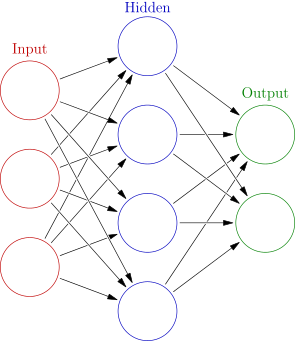
\includegraphics[scale=0.6]{pictures/neural_network.png}
	\caption{An artificial neural network is an interconnected group of nodes, akin to the vast network of neurons in a brain. Here, each circular node represents an artificial neuron and an arrow represents a connection from the output of one artificial neuron to the input of another\cite{NNPIC}.}
	\label{fig:1}
\end{figure}

\subsection{Weight Matrix and Bias Vector}
In the inner formula of each neuron $h=\sigma(Wx+b)$, we have two network parameters $W$ and $b$ inside the activation function $\sigma()$. They are the weight matrix and bias vector respectively. Each layer (neuron) has its own weight matrix and bias vector. For a neural networks with $n$ layers, we have totally $n$ pairs of such parameters, $[W^1, W^2,...,W^n]$ and $[b^1,b^2,...,b^n]$. The dimensions of each $W^i$ and $b^i$ are determined by the dimensions of the input and output values in each layer. For example, suppose the input \(x\in \mathbb{R}^{d}\) and the layer maps it to \(h\in \mathbb{R}^{p}\). In this case, the weight matrix $W^i$ functions to map data from $\mathbb{R}^{d}$ to $\mathbb{R}^{p}$, so it is a $p \times d$ matrix. The bias vector $b^i$ is a vector with length $p$.

\subsection{Non-linear Activation Function}
If we apply the two linear projection functions $h=W^1x+b^1$ and $z'=W^2x+b^2$ and the cost function is Euclidean distance $\norm{x-x'}_2$, this two-layer neural network is identical to the PCA. However, most people are attracted by the nonlinear aspect of the autoencoders, which makes it effective in solving more real-life problems.\\
To introduce non-linearity into ANN, we apply element-wise non-linear functions such as a sigmoid function or a rectified linear unit after linear projections. The non-linear function in each neuron is $h= f(Wx + b)$ where the non-linear mapping $f$ acts as the activation function. The commonest activation function is sigmoid function $f(t)=\dfrac{1}{1+e^{-t}}$. We use $\sigma()$ to represent this sigmoid function. Thus each layer within an ANN consists a function \(h=\sigma(Wx+b)\), taking input \(x\in \mathbb{R}^{d}\) and mapping it to \(z\in \mathbb{R}^{p}\).
\begin{figure}[H]
	\centering
	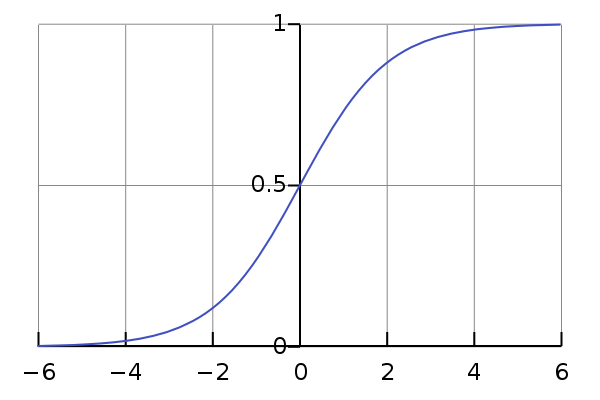
\includegraphics[scale=0.4]{pictures/sigmoid.png}
	\caption{Logistic curve $f(t)=\dfrac{1}{1+e^{-t}}$\cite{SIGPIC}.}
	\label{fig:2}
\end{figure}


\section{Autoencoders}
An autoencoder is an artificial neural network used for unsupervised learning of efficient codings. The aim of an autoencoder is to learn a representation (encoding) for a set of data, typically for the purpose of dimensionality reduction. Autoencoders are simple learning circuits which aim to transform inputs into outputs with the least possible amount of distortion. While conceptually simple, they play an important role in machine learning. Recently, autoencoders have taken center stage again in the “deep architecture” approach and this concept has become more widely used for learning generative models of data\cite{AE, AE3}.\\
\begin{figure}[H]
	\centering
	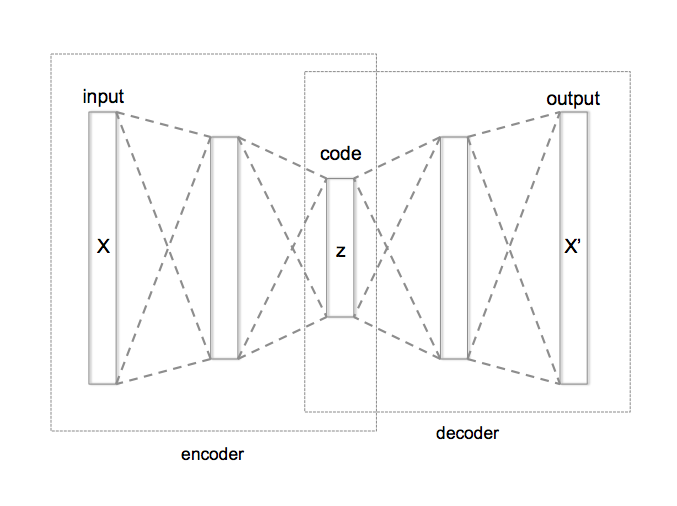
\includegraphics[scale=0.6]{pictures/Autoencoder_structure.png}
	\caption{Schematic structure of an autoencoder with 3 fully-connected hidden layers\cite{AEPIC}.}
	\label{fig:3}
\end{figure}
Typically, an autoencoder consists two parts, an encoding phase (encoder) \(E(\cdot)\) and an decoding phase (decoder) \(D(\cdot)\). The encoder \(E(\cdot)\) receives input data and outputs mid-layer-data, which acts as the input data for the decoder \(D(\cdot)\). The decoder maps the mid-layer-data back to the original feature space. The encoder and decoder can be comprised of single layer or multiple layers, each layer with a function \(z=\sigma(Wx+b)\) mapping \(x\in \mathbb{R}^{d}\) to \(z\in \mathbb{R}^{p}\).  \(\sigma\) is an element-wise activation function such as a sigmoid function or a rectified linear unit. A typical autoencoder structure is shown as following:\\
In the simplest case, where there is one hidden layer, the encoder stage of an autoencoder maps \(x\in \mathbb{R}^{d}=\mathcal{X}\) to \(z\in \mathbb{R}^{p}=\mathcal{F}\) ($z$ is hidden layer, for this simplest case, it is also the mid-layer of the whole autoencoder). The encoder \(E(\cdot)\) and the decoder \(D(\cdot)\) can be defined as transitions $\phi$ and $\psi$,
\begin{equation}
\begin{split}
& \phi:\mathcal{X}\to\mathcal{F} \\
& \psi:\mathcal{F}\to\mathcal{X} \\
& \phi,\psi=\operatorname*{argmin}_{\phi,\psi} \norm{X-(\phi \circ \psi)X}^2
\end{split}
\end{equation}
This can be written as
\begin{equation}
z=\sigma(Wx+b)
\end{equation}
The image $z$ is usually referred to as code, latent variables, or latent representation. Here, $\sigma()$ is an element-wise activation function such as a sigmoid function or a rectified linear unit. $W$ is a weight matrix and $b$ is a bias vector. The decoder stage of the autoencoder maps $z$ to the reconstruction $x'$  of the same shape and in the same dimension with original data $x$:
\begin{equation}
x'=\sigma'(W'z+b')
\end{equation}
where $\sigma'$, $W'$ and $b'$ for the decoder may differ in general from the corresponding $\sigma$, $W$ and $b$ for the encoder, depending on the design of the autoencoder.\\
In the training process, autoencoders are usually trained to minimize reconstruction errors (such as squared errors) between original $x$ and the reconstructed $x'$:
\begin{equation}
\mathcal{L}(x,x')=\norm{x-x'}^2=\norm{x-\sigma'(W'(\sigma(Wx+b))+b')}^2
\end{equation}
where $x$ is usually averaged over some input training set\cite{AE}.

\section{Canonical Correlation Analysis}
In statistics, Canonical Correlation Analysis (CCA) is a way of inferring information from cross-covariance matrices. If we have two vectors \(X = (X_{1}, ..., X_{n})\) and \(Y = (Y_{1}, ..., Y_{m})\) of random variables, and there are correlations among the variables, then CCA will find linear combinations of the $X_{i}$ and $Y_{j}$ which have maximum correlation with each other\cite{CCA}. From \cite{ECCA}, we derive the following formulas to explain this algorithm.\\
Consider two random vectors $x\in \mathbb{R}^{m}$ and $y\in \mathbb{R}^{n}$. Let $z= \begin{bmatrix}x^T & y^T\end{bmatrix}^T \in \mathbb{R}^{m+n}$. We assume that x and y have zero means and share the nonsingular composite covariance matrix
\begin{equation}
R_{zz}=E[zz^T]=\begin{bmatrix}
R_{xx} & R_{xy} \\
R_{xy} & R_{yy}
\end{bmatrix}
\end{equation}
where the elements of the cross-covariance matrix $R_{xy}$ are inner products in Hilbert space of second-order random variables. $R_{xy}[i,j]=E[x_{i}y_{j}]$ is the inner product between random variables $x_{i}$ and $y_{j}$ in the Hilbert space. \\
The coherence matrix of $x$ and $y$ is defined as
\begin{equation}
C=E[(R_{xx}^{-1/2}x)(R_{yy}^{-1/2}y)^T]=R_{xx}^{-1/2}R_{xy}R_{yy}^{-T/2}
\end{equation}
A singular value decomposition (SVD) for the coherence matrix $C$ may be written as
\begin{equation}
\begin{split}
C=R_{xx}^{-1/2}R_{xy}R_{yy}^{-T/2}=F\Sigma G^T, \\ F^TCG=F^TR_{xx}^{-1/2}R_{xy}R_{yy}^{-T/2}G=\Sigma
\end{split}
\end{equation}
where $F\in \mathbb{R}^{m\times m}$ and $G\in \mathbb{R}^{n\times n}$ are orthogonal matrices and the matrix $\Sigma$ is a diagonal singular value matrix with $\Sigma(m)=diag[\sigma_{1},\sigma_{2},...,\sigma_{m}]$; $\sigma_{1}\geq\sigma_{2}\geq...\geq\sigma_{m}>0$. Let the elements of $u\in \mathbb{R}^{m}$ and $v\in \mathbb{R}^{n}$ be the canonical coordinates of $x$ and $y$. \\
The diagonal matrix
\begin{equation}
\Sigma=F^TCG=F^TR_{xx}^{-1/2}R_{xy}R_{yy}^{-T/2}G=E[(F^TR_{xx}^{-1/2}x)(G^TR_{yy}^{-T/2}y)^T]=E[uv^T]
\end{equation}
is the canonical correlation matrix. Each $\sigma_{i}$ is the correlation between pairs of canonical coordinates $(u_{i},v_{i})$. \\
From the above equation, we extract the following expression for canonical variables $u$ and $v$:
\begin{equation}
u=F^TR_{xx}^{-1/2}x,\quad v=G^TR_{yy}^{-T/2}y
\end{equation}
The standard measure of linear dependence for the composite vector is the Hadamard ratio where the ratio takes the value 0 if and only if there is linear dependence among the elements of the composite vector and takes the value 1 if and only if elements of the composite vector are mutually uncorrelated. \\
In the paper, the author made a decomposition of the Hadamard ratio and derived the following term
\begin{equation}
L=det(I-\Sigma\Sigma^T)=\prod_{i=1}^{m}(1-\sigma_{i}^2);\quad 0\leq L\leq 1
\end{equation}
which measures the linear dependence between $x$ and $y$. Correspondingly,
\begin{equation}
H=1-L=1-det(I-\Sigma\Sigma^T)=1-\prod_{i=1}^{m}(1-\sigma_{i}^2);\quad 0\leq H\leq 1
\end{equation}
measures the linear coherence between $x$ and $y$.

\section{Kernel Methods}
Kernel methods owe their name to the use of kernel functions, which enable them to operate in a high-dimensional, implicit feature space without ever computing the coordinates of the data in that space, but rather by simply computing the inner products between the images of all pairs of data in the feature space. This operation is often computationally cheaper than the explicit computation of the coordinates. This approach is called the ``kernel trick"\cite{PR}. Given $x_{i}$ and $y_{j}$, the function $K(x_{i},y_{j}): \mathbb{R} \times \mathbb{R} \to \mathbb{R}$ is often referred to a kernel function.
\begin{figure}[H]
	\centering
	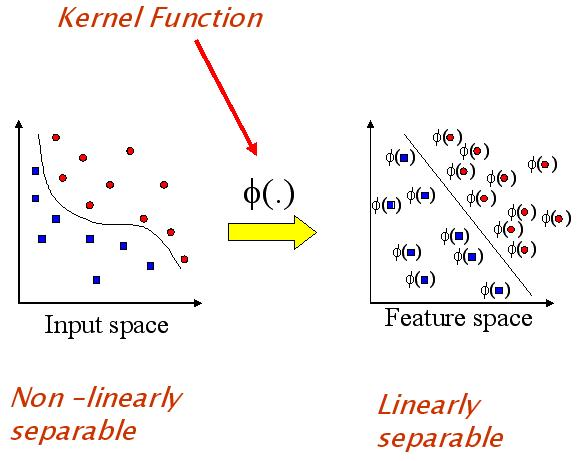
\includegraphics[scale=0.6]{pictures/kernel.jpg}
	\caption{A visual demonstration of kernel function. A kernel function maps data from original feature space to a higher dimensional space and avoids the explicit mapping that is needed to get linear learning algorithms to learn a nonlinear function or decision boundary\cite{KPIC}.}
	\label{fig:4}
\end{figure}

\subsection{Positive Definite Kernel}
A positive definite kernel is a generalization of a positive definite function or a positive definite matrix. It makes sure there is a corresponding inner product space for $x$ and $y$. Its greatest advantage is that positive definite kernels can be defined on every set. Therefore it can be applied to data of any type.\\
Certain problems in machine learning have additional structure than an arbitrary weighting function $K$. The computation is made much simpler if the kernel can be written in the form of a "feature map" $\varphi:\mathcal{X}\to\mathcal{V}$ which satisfies $K(x,x')=\langle \varphi (x), \varphi (x') \rangle \mathcal{V}$. The key restriction is that $\langle \cdot, \cdot \rangle \mathcal{V}$ must be a proper inner product. On the other hand, an explicit representation for $\varphi$ is not necessary, as long as $\mathcal{V}$ is an inner product space\cite{PD}.\\
In KPCA or KCCA, a kernel function maps data from original space to an inner product space RKHS to ensure both the existence of an inner product and the evaluation of every function in this space at every point in the domain. From the definition of RKHS, the corresponding kernel function should be both symmetric and positive definite\cite{RKHS}.

\subsection{Mercer's Theorem}
To explore a kernel function $K$ without the explicit representation for $\varphi$, we apply Mercer's theorem: an implicitly defined function $\varphi$ exists whenever space $\mathcal {X}$ can be equipped with a suitable measure ensuring the function $K$ satisfies Mercer's condition.\\
In mathematics, specifically functional analysis, Mercer's theorem is a representation of a symmetric positive definite function on a square as a sum of a convergent sequence of product functions. This theorem, presented in (Mercer 1909), is one of the most notable results of the work of James Mercer\cite{MT}.
To explain Mercer's theorem, we first consider an important special case; see below for a more general formulation. A kernel, in this context, is a symmetric continuous function
\begin{equation}
K:[a,b] \times [a,b] \rightarrow \mathbb {R}
\end{equation}
where symmetric means that \( K(x, s) = K(s, x)\).
K is said to be non-negative definite (or positive semidefinite) if and only if
\begin{equation}
\sum _{i=1}^{n}\sum _{j=1}^{n}K(x_{i},x_{j})c_{i}c_{j}\geq 0
\end{equation}

\subsection{Schoenberg's Theroem}
Suppose a kernel function $K$ is not positive definite, it may not represent an inner product in any Hilbert space. Here is one way to see. A kernel $K$ is positive definite if and only if for all samples of n points, its corresponding kernel matrix $\mathcal{K}$ is a positive definite matrix. With a positive definite $\mathcal{K}$, by Cholesky decompose $\mathcal{K}=LL^T$, each row of $L$ as one mapped point in the inner product space. If $K$ is not positive definite, the matrix $\mathcal{K}$ may also not be positive definite. Consequently, Cholesky does not work and there is no corresponding inner product space. \\
\textbf{Definition.} A function $f$ with domain $(0, \infty)$ is said to be completely monotonic, if it possesses derivatives $f^{(n)}(x)$ for all $n=0,1,2,3,...$ and if $(-1)^nf^{(n)}(x) \geq 0$\cite{CMF}. \\
Schoenberg\cite{Schoenberg} provides a method to ensure the kernel function to be positive definite: If \(f(t)\) is a completely monotonic function, then the radial kernel
\begin{equation}
K(x,y)=f(\norm{x-y}^2)
\end{equation}
is positive definite on any Hilbert space. Since the radial kernel is already symmetric, the above Schoenberg's theorem provides us a direct way to get a symmetric positive definite kernel function satisfying RKHS definition for our model.

\section{KCCA}
In section 2.3, we explain CCA step by step. For two random vectors $x\in R^{m}$ and $y\in R^{n}$, let $z= \begin{bmatrix}x^T & y^T\end{bmatrix}^T \in R^{m+n}$ and assume that x and y have zero means. formula 2.7 is the covariance matrix of $x$ and $y$. The elements of the cross-covariance matrix $R_{xy}$ are inner products in Hilbert space of second-order random variables. $R_{xy}[i,j]=E[x_{i}y_{j}]$ is the inner product between random variables $x_{i}$ and $y_{j}$ in the Hilbert space. To leverage the power of non-linearity, we apply kernel methods to CCA. As in the linear case, the aim of KCCA is to find canonical variables of the input data. Thus we derive its calculation based upon the formulas for CCA in section 2.3. \\
Here, to obtain the covariance matrix of $x$ and $y$ in RKHS, we define
\begin{equation}
\begin{split}
R_{xx}[i,j] = K(x_{i},x_{j}) \\
R_{xy}[i,j] = K(x_{i},y_{j}) \\
R_{yx}[i,j] = K(y_{i},x_{j}) \\
R_{yy}[i,j] = K(y_{i},y_{j})
\end{split}
\end{equation}
where $K(x_{i},y_{j}): \mathbb{R} \times \mathbb{R} \to \mathbb{R}$ is a positive definite kernel function. Thus the covariance matrix becomes
\begin{equation}
\begin{split}
R_{zz}={} & \begin{bmatrix}
R_{xx} & R_{xy} \\
R_{xy} & R_{yy}
\end{bmatrix}= \\
& \begin{bmatrix}
\begin{pmatrix}
K(x_{1},x_{1}) & \dots & K(x_{1},x_{m})\\ \vdots & \ddots & \\ K(x_{m},x_{1}) & & K(x_{m},x_{m})
\end{pmatrix} &
\begin{pmatrix}
K(x_{1},y_{1}) & \dots & K(x_{1},y_{n})\\ \vdots & \ddots & \\ K(x_{m},y_{1}) & & K(x_{m},y_{n})
\end{pmatrix} \\
\begin{pmatrix}
K(y_{1},x_{1}) & \dots & K(y_{1},x_{m})\\ \vdots & \ddots & \\ K(y_{n},x_{1}) & & K(y_{n},x_{m})
\end{pmatrix} &
\begin{pmatrix}
K(y_{1},y_{1}) & \dots & K(y_{1},y_{n})\\ \vdots & \ddots & \\ K(y_{n},y_{n}) & & K(y_{n},y_{n})
\end{pmatrix}
\end{bmatrix}
\end{split}
\end{equation}
where the elements of the cross-covariance matrix $R_{xy}$ are inner products in the RKHS of random variables $x$ and $y$. $R_{xy}[i,j]=K(x_{i},y_{j})$ is the inner product between random variables $x_{i}$ and $y_{j}$ in the RKHS. \\
We mimic all the remaining formulas from 2.8 to 2.13, except that, with kernel methods, $L$ and $H$ now measure the non-linear dependence and non-linear coherence between $x$ and $y$ respectively.

\section{Principal Component Analysis}
Principal Component Analysis (PCA) is a popular unsupervised learning approach for discovering a low-dimensional set of features from a large set of variables. For high-dimensional data, principal components allow us to summarize this set with a smaller number of representative variables that collectively explain most of the variability in the original set. PCA refers to the process by which principal components are computed, and the subsequent use of these components in understanding the data. The first principal component of a set of features \(X = (X_{1}, X_{2},..., X_{p})\) is the normalized linear combination of the features
\begin{equation}
Z_{1} = \phi_{11}X_{1} + \phi_{21}X_{2} +...+ \phi_{p1}X_{p}
\end{equation}
that has the largest variance. After the first principal component \(Z_{1}\) of the features has been determined, we can find the second principal component \(Z_{2}\). The second principal component is the linear combination of \(X = (X_{1}, X_{2},..., X_{p})\) that has maximal variance out of all linear combinations that are uncorrelated with \(Z_{1}\). The third principal component is the linear combination of \(X = (X_{1}, X_{2},..., X_{p})\) that has maximal variance out of all linear combinations that are uncorrelated with \(Z_{1}\) and \(Z_{2}\). So on and so forth\cite{STAT}. \\
Finally, we will have totally p unique principal components \(Z_{1}, Z_{2},..., Z_{p}\). Each unique principal component \(Z_{i}\) explains a specific percentage of variance to the original dataset, a positive quantity, ranging from 0 to 1. And the percentages of all p principal components sum to 1. In most programming PCA tools, the principal components appear with a descending order of the percentages by variance they explain. These percentages are cumulative, indicating the cumulative variance explained to the original dataset by their corresponding principal components. Thus, to understand the data and execute proceeding analysis after PCA, we typically extract first k principal components \(Z_{1}, Z_{2},..., Z_{k}, k <p \). These k principal components usually explain most of the variance of the original data, above 90\% or 95\%.

\chapter{Model Design}
In section 2.1 and 2.2, we described how autoencoders learn through training and finally reconstruct data $x$ back to its original space, with minimal reconstruction errors. Herein we try to modify this task that given input dataset $x$, we want the model to reconstruct another "potentially correlated dataset" $y$. From initial experiments on autoencoders, we found that the reconstruction results were mediocre. The main reason is that an autoencoder does not have training process on extracting the correlation between the two datasets $x$ and $y$. Instead, it merely explores ``direct mapping" from one cluster of patterns to another one. This leads to devastating issues in reconstruction results (In next chapter, we will use some image examples to demonstrate the issues). To avoid such issues and accomplish the new task, we introduce KCCA to dig out the correlations between the pair of input data sets and create a novel model KCE.  \\
In this chapter, we will introduce three models, the \textit{Non-Coherence Encoder (NCE)}, the \textit{Coherence Encoder (CE)} and the \textit{Kernel Coherence Encoder (KCE)} as well as their theoretical details. The NCE is designed without CCA and coherence. In this model, the connection between the two data sets is explored exclusively through deep learning. The CE model, based upon the NCE and modified by applying linear CCA within its encoder phase, outputs linear canonical variables to the decoder phase. The KCE model, which is the ultimate model of the thesis research, substitutes the linear CCA in CE with KCCA thus extending the encoder phase to a non-linear stage. Notably, the decoder phases for these three models have exactly the same structures. 

\section{Non-Coherence Encoder (NCE)}
This section is a general introduction of our model NCE. The flowchart in figure 3.1 provides a step-by-step description of the model. The model is divided into two phases, encoder phase, and decoder phase. Though having a very different structure with an autoencoder, it maintains its major properties: dimension reduction, non-linear mapping, and reconstruction error minimization. The encoder phase reduces the dimension of input data, while the decoder phase maps data back to their original spaces and finish the reconstruction.We are going to explain their functionalities and structures in detail. 
\begin{figure}[H]
	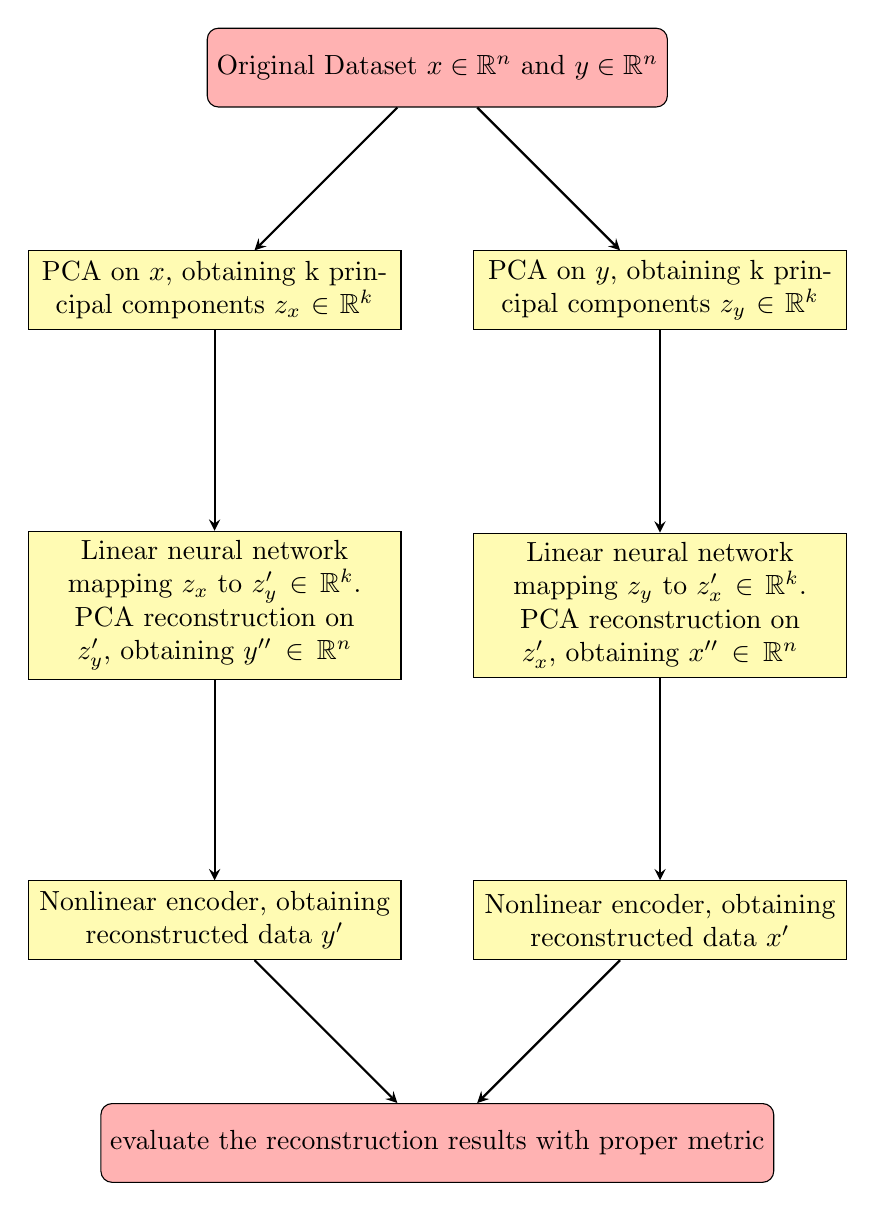
\begin{tikzpicture}[node distance=4cm]
	
	\node (p1) [startstop] {Original Dataset $x\in \mathbb{R}^{n}$ and $y\in \mathbb{R}^{n}$};
	\node (p2) [process, below left of = p1] {PCA on $x$, obtaining k principal components $z_x\in \mathbb{R}^{k}$};
	\node (p3) [process, below right of = p1] {PCA on $y$, obtaining k principal components $z_y\in \mathbb{R}^{k}$};
	
	\draw [arrow] (p1) -- (p2);
	\draw [arrow] (p1) -- (p3);
	
	\node (p5) [process, below of = p2] {Linear neural network mapping $z_x$ to $z_y'\in \mathbb{R}^{k}$. PCA reconstruction on $z_y'$, obtaining $y''\in \mathbb{R}^{n}$};
	\node (p6) [process, below of = p3] {Linear neural network mapping $z_y$ to $z_x'\in \mathbb{R}^{k}$. PCA reconstruction on $z_x'$, obtaining $x''\in \mathbb{R}^{n}$};
	
	\draw [arrow] (p2) -- (p5);
	\draw [arrow] (p3) -- (p6);
	
	\node (p7) [process, below of = p5] {Nonlinear encoder, obtaining reconstructed data $y'$};
	\node (p8) [process, below of = p6] {Nonlinear encoder, obtaining reconstructed data $x'$};
	
	\draw [arrow] (p5) -- (p7);
	\draw [arrow] (p6) -- (p8);
	
	\node (p9) [startstop, below right of = p7] {evaluate the reconstruction results with proper metric};
	
	\draw [arrow] (p7) -- (p9);
	\draw [arrow] (p8) -- (p9);
	
	
	\end{tikzpicture}
	\centering
	\caption{Flow chart of the model NCE}
	\label{fig:1}
\end{figure}

\subsection{Encoder Phase}
The only step in the encoder phase of the model NCE is PCA. We reduce the dimension of the original data to a low-dimensional space where the principal components contain most information of the data. \\

\textbf{PCA}\\
In real-life problems, data $x\in \mathbb{R}^{n}$ and $y\in \mathbb{R}^{n}$ are usually high-dimensional data. We have two concerns with this issue: First, directly using the high-dimensional data as input data will slow down the ANN, and moreover, cause over-fitting\cite{STAT}, making our model neither efficient nor effective. Second, for the subsequent step KCCA, we need to calculate the determinant of the kernel covariance matrix (Gramian matrix) $R_{zz} \in \mathbb{R}^{2n} \times \mathbb{R}^{2n}$. From experimental trials, we find that high-dimensional Gramian matrix is easy to become singular (not invertible) in the new space thus impossible to calculate its determinant.\\
So we apply PCA to reduce the dimensions of original data before using KCCA. As we described in chapter 2, PCA is a dimension reduction algorithm that allows us to summarize high-dimensional data set with a smaller number of representative variables that collectively explain most of the variability in the original set. PCA refers to the process by which principal components are computed, and the subsequent use of these components in understanding the data.\\
To reach a trade-off between model accuracy and the above two concerns, we take the first k principal components \(Z_{1}, Z_{2},..., Z_{k}\) that explain over 90\% variance of the original data, where $k$ is a much smaller integer compared with the original dimension $n$. As a result, the input data for the KCCA step become $z_x\in \mathbb{R}^{k}$ and $z_y\in \mathbb{R}^{k}$. Meanwhile, we keep the eigenvectors and means of $x$ and $y$ generated in this step for PCA reconstruction.

\subsection{Decoder Phase}
The encoder phase of the model NCE applies neither KCCA nor CCA. Thus the decoder phase of NCE maps $z_x$ to $y'$ and $z_y$ to $x'$ through by three steps: linear ANNs, PCA reconstruction, and non-linear ANNs.\\

\textbf{Linear ANNs}\\
The first step for the decoder phase is to transfer the canonical variables $u$ and $v$ to the spaces of principle components $z_y$ and $z_x$ respectively. Here we use 2 two-layer linear ANNs to map $u$ and $v$ to $z_y{'}$ and $z_x{'}$. The two ANNs are namely $\gamma_1$ and $\gamma_2$:
\begin{equation}
\begin{split}
&z_y^{'}=W_{1,2}(W_{1,1}u+b_{1,1})+b_{1,2} \\
&z_x^{'}=W_{2,2}(W_{2,1}v+b_{2,1})+b_{2,2} \\
&\gamma_1(W_{1,1},W_{1,2},b_{1,1},b_{1,2})=\operatorname*{argmin}_{W_{1,1},W_{1,2},b_{1,1},b_{1,2}}\norm{z_y-z_y^{'}}^2 \\
&\gamma_2(W_{2,1},W_{2,2},b_{2,1},b_{2,2})=\operatorname*{argmin}_{W_{2,1},W_{2,2},b_{2,1},b_{2,2}}\norm{z_x-z_x^{'}}^2
\end{split}
\end{equation}
$\gamma_1$ and $\gamma_2$ provide us $z_y^{'}$ and $z_x^{'}$ which have minimal difference with $z_y$ and $z_x$ respectively.\\

\textbf{PCA Reconstruction}\\
Then we need an operation that maps the principal components $z_x$ and $z_y$ back to the original feature space of $y$ and $x$. Our solution is PCA reconstruction, which can be thought as the ``reverse" PCA that maps principal components to high-dimensional feature space.
\begin{equation}
PCA\ reconstruction=PC\ scores \cdot Eigenvectors^T + Mean
\end{equation}
Eigenvectors map the principal components $z\in \mathbb{R}^{k}$ back to the original feature space $x^{'}\in \mathbb{R}^{n}$. We make use of the eigenvectors and means of $y$ and $x$ that we obtain in the first PCA step and follow 3.11 to get the PCA reconstruction.
\begin{equation}
\begin{split}
y''= z_y^{'}\cdot Eigenvectors_{y}^T + Mean_y \\
x''= z_x^{'}\cdot Eigenvectors_{x}^T + Mean_x
\end{split}
\end{equation}

\textbf{Non-linear ANNs}\\
From experimental results, we found that the results of PCA reconstruction, $y''$ and $x''$, though in the feature space of $y$ and $x$, are not precise enough to be the final results. On the one hand, training errors are unavoidable in ANNs. The previous training processes are all executed to principal components in the lower-dimensional spaces $\mathbb{R}^{k}$. The last mappings from $\mathbb{R}^{k}$ to $\mathbb{R}^{n}$ amplify the dimensions of data as well as the reconstruction errors. On the other hand, we mentioned that the k principal components explain over 90\% variances. This means that during PCA and PCA reconstruction, a small part of the information from the original data gets lost. For these two reasons, we need one more training step where the errors are computed in the feature spaces of original data sets to enhance the performance of our model. \\
This training process for our model is 2 two-layer non-linear encoders mapping $y''$ to $y'$ and $x''$ to $x'$ respectively. It minimizes the error between $y'$ and original data $y$ and error between $x'$ and original data $x$. Slightly different from typical autoencoders that are usually trained to minimize reconstruction errors (such as squared errors) between input data and its own reconstructed data, our encoders are trained to minimize reconstruction error between $y$ and $y'$ and reconstruction error between $x$ and $x'$ (note that the input data of this step are not $y$ and $x$, but $y''$ and $x''$). We define the two ANNs as $\mathcal{E}_1$ and $\mathcal{E}_2$:
\begin{equation}
\begin{split}
&y'=W_{1,3}(W_{1,4}y''+b_{1,3})+b_{1,4} \\
&x'=W_{2,3}(W_{2,4}x''+b_{2,3})+b_{2,4} \\
&\mathcal{E}_1(W_{1,3},W_{1,4},b_{1,3},b_{1,4})=\operatorname*{argmin}_{W_{1,3},W_{1,4},b_{1,3},b_{1,4}}\norm{y-y'}^2 \\
&\mathcal{E}_2(W_{2,3},W_{2,4},b_{2,3},b_{2,4})=\operatorname*{argmin}_{W_{2,3},W_{2,4},b_{2,3},b_{2,4}}\norm{x-x'}^2
\end{split}
\end{equation}
This is the last step of the whole model. Once the training errors converge, we obtain reconstruction $y'$ and $x'$ and evaluate the model performance.

\section{Coherence Encoder (CE)}
This section is a general introduction to our model CE. The flowchart in figure 3.2 provides a step-by-step description of the model. The model CE also has encoder phase and decoder phase, while comparing with NCE, the encoder phase contains one more CCA step and the decoder phase remains consistent.  
\begin{figure}[H]
	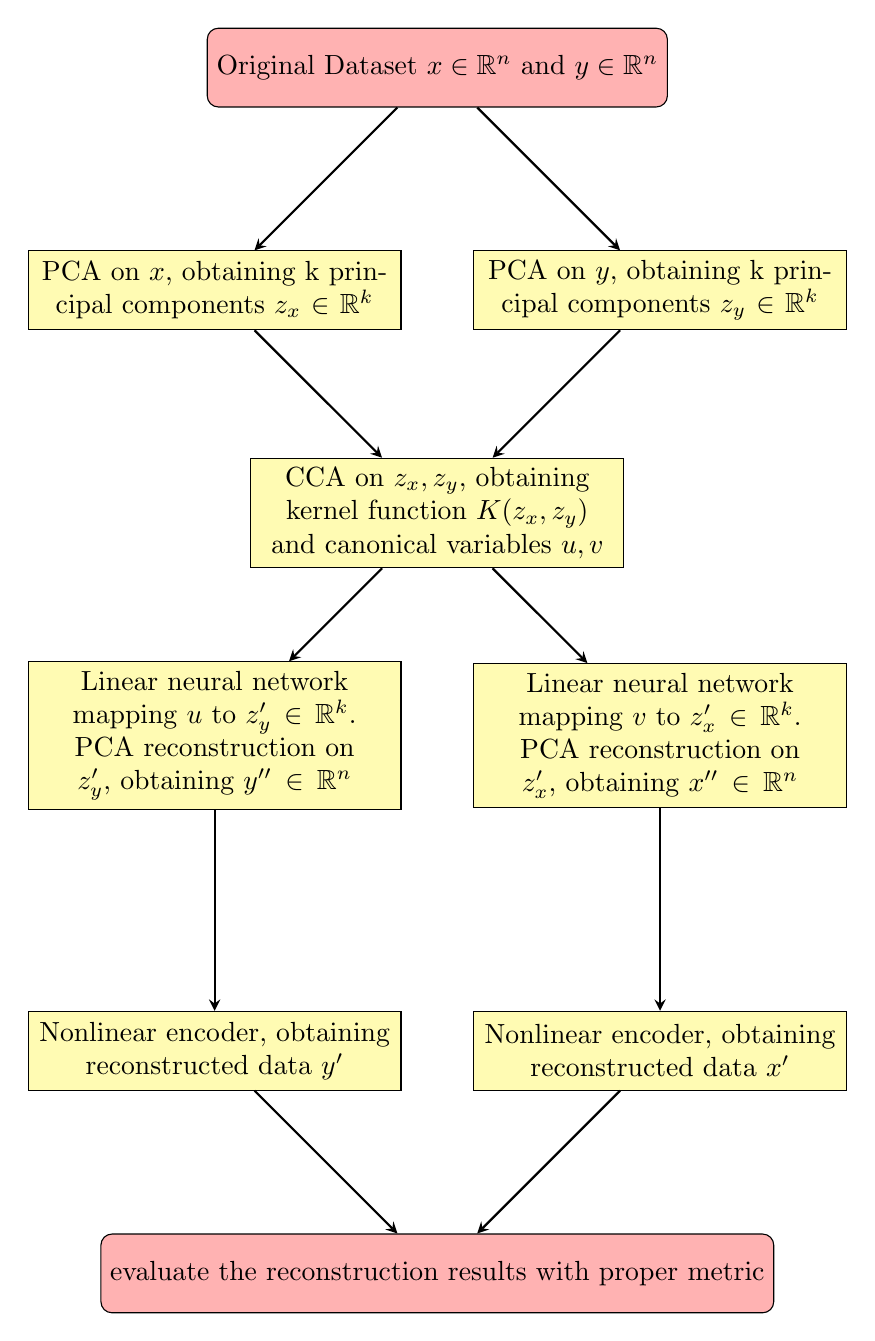
\begin{tikzpicture}[node distance=4cm]
	
	\node (p1) [startstop] {Original Dataset $x\in \mathbb{R}^{n}$ and $y\in \mathbb{R}^{n}$};
	\node (p2) [process, below left of = p1] {PCA on $x$, obtaining k principal components $z_x\in \mathbb{R}^{k}$};
	\node (p3) [process, below right of = p1] {PCA on $y$, obtaining k principal components $z_y\in \mathbb{R}^{k}$};
	
	\draw [arrow] (p1) -- (p2);
	\draw [arrow] (p1) -- (p3);
	
	\node (p4) [process, below right of = p2] {CCA on $z_x,z_y$, obtaining kernel function $K(z_x, z_y)$ and canonical variables $u,v$};
	
	\draw [arrow] (p2) -- (p4);
	\draw [arrow] (p3) -- (p4);
	
	\node (p5) [process, below left of = p4] {Linear neural network mapping $u$ to $z_y'\in \mathbb{R}^{k}$. PCA reconstruction on $z_y'$, obtaining $y''\in \mathbb{R}^{n}$};
	\node (p6) [process, below right of = p4] {Linear neural network mapping $v$ to $z_x'\in \mathbb{R}^{k}$. PCA reconstruction on $z_x'$, obtaining $x''\in \mathbb{R}^{n}$};
	
	\draw [arrow] (p4) -- (p5);
	\draw [arrow] (p4) -- (p6);
	
	\node (p7) [process, below of = p5] {Nonlinear encoder, obtaining reconstructed data $y'$};
	\node (p8) [process, below of = p6] {Nonlinear encoder, obtaining reconstructed data $x'$};
	
	\draw [arrow] (p5) -- (p7);
	\draw [arrow] (p6) -- (p8);
	
	\node (p9) [startstop, below right of = p7] {evaluate the reconstruction results with proper metric};
	
	\draw [arrow] (p7) -- (p9);
	\draw [arrow] (p8) -- (p9);
	
	\end{tikzpicture}
	\centering
	\caption{Flow chart of the model CE}
	\label{fig:2}
\end{figure}

\subsection{Encoder Phase}
In the encoder phase of the model CE, we apply linear CCA to extract the connection between the two datasets. More precisely, we do CCA on the principal components of the original data.\\ 

\textbf{PCA}\\
This step is exactly the same with PCA step in NCE. It takes original data $x\in \mathbb{R}^{n}$ and $y\in \mathbb{R}^{n}$ and generates their principal components $z_x\in \mathbb{R}^{k}$ and $z_y\in \mathbb{R}^{k}$.\\

\textbf{CCA}\\
In this step, we apply CCA to extract the correlation between two sets of principal components. As a result of CCA, we obtain the canonical variables $u$ and $v$, corresponding to $z_x$ and $z_y$. \\
The calculation is based upon section 2.3. Given principal components $z_x\in \mathbb{R}^{k}$ and $z_y\in \mathbb{R}^{k}$. Let $z= \begin{bmatrix}x^T & y^T\end{bmatrix}^T \in \mathbb{R}^{n2k}$. We obtain the following covariance matrix
\begin{equation}
R_{zz}=E[zz^T]=\begin{bmatrix}
R_{z_{x}z_{x}} & R_{z_{x}z_{y}} \\
R_{z_{x}z_{y}} & R_{z_{y}z_{y}}
\end{bmatrix}
\end{equation}
The remaining calculations follows formulas 2.8 to 2.11, until we get that canonical variables $u$ and $v$,
\begin{equation}
u=F^TR_{xx}^{-1/2}x,\quad v=G^TR_{yy}^{-T/2}y
\end{equation}

\subsection{Decoder Phase}
As we mentioned earlier, the decoder phase of the CE shares exactly the same structure with the decoder phase of NCE. The only difference is that here we take canonical variables $u$ and $v$ as the input of the decoder phase. 

\section{Kernel Coherence Encoder (KCE)}
This section is a general introduction of our model KCE. The flowchart in figure 3.3 provides a step-by-step description of the model. The encoder phase of the model KCE takes advantage of KCCA and includes a training process to optimize the kernel function. 
\begin{figure}[H]
	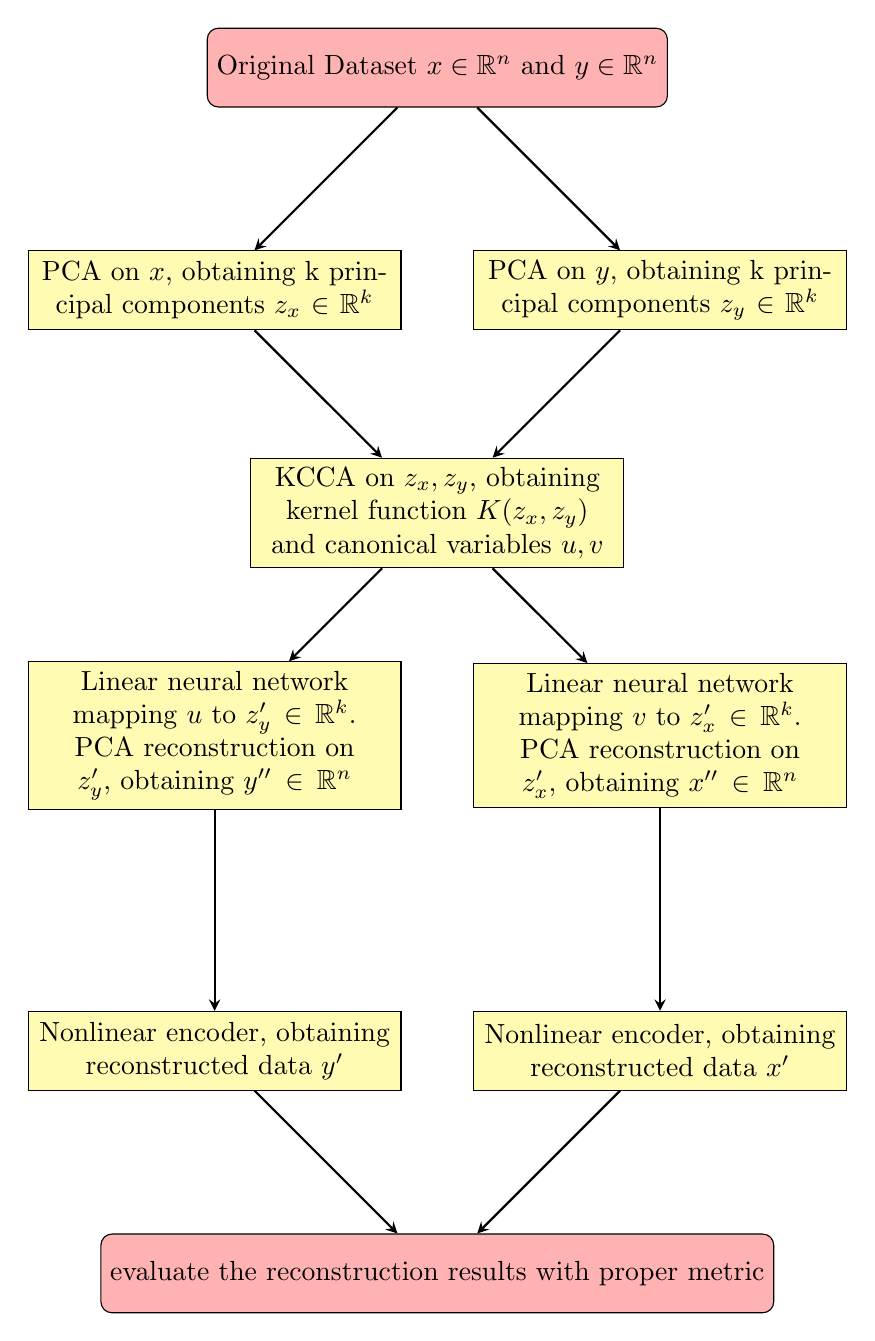
\begin{tikzpicture}[node distance=4cm]
	
	\node (p1) [startstop] {Original Dataset $x\in \mathbb{R}^{n}$ and $y\in \mathbb{R}^{n}$};
	\node (p2) [process, below left of = p1] {PCA on $x$, obtaining k principal components $z_x\in \mathbb{R}^{k}$};
	\node (p3) [process, below right of = p1] {PCA on $y$, obtaining k principal components $z_y\in \mathbb{R}^{k}$};
	
	\draw [arrow] (p1) -- (p2);
	\draw [arrow] (p1) -- (p3);
	
	\node (p4) [process, below right of = p2] {KCCA on $z_x,z_y$, obtaining kernel function $K(z_x, z_y)$ and canonical variables $u,v$};
	
	\draw [arrow] (p2) -- (p4);
	\draw [arrow] (p3) -- (p4);
	
	\node (p5) [process, below left of = p4] {Linear neural network mapping $u$ to $z_y'\in \mathbb{R}^{k}$. PCA reconstruction on $z_y'$, obtaining $y''\in \mathbb{R}^{n}$};
	\node (p6) [process, below right of = p4] {Linear neural network mapping $v$ to $z_x'\in \mathbb{R}^{k}$. PCA reconstruction on $z_x'$, obtaining $x''\in \mathbb{R}^{n}$};
	
	\draw [arrow] (p4) -- (p5);
	\draw [arrow] (p4) -- (p6);
	
	\node (p7) [process, below of = p5] {Nonlinear encoder, obtaining reconstructed data $y'$};
	\node (p8) [process, below of = p6] {Nonlinear encoder, obtaining reconstructed data $x'$};
	
	\draw [arrow] (p5) -- (p7);
	\draw [arrow] (p6) -- (p8);
	
	\node (p9) [startstop, below right of = p7] {evaluate the reconstruction results with proper metric};
	
	\draw [arrow] (p7) -- (p9);
	\draw [arrow] (p8) -- (p9);
	
	
	\end{tikzpicture}
	\centering
	\caption{Flow chart of our KCE model}
	\label{fig:3}
\end{figure}

\subsection{Encoder Phase}
In the encoder phase of the model KCE, we apply KCCA to extract the connection between the two datasets. \\

\textbf{PCA}\\
This step is exactly the same with PCA step in the models NCE and CE. It takes original data $x\in \mathbb{R}^{n}$ and $y\in \mathbb{R}^{n}$ and generates their principal components $z_x\in \mathbb{R}^{k}$ and $z_y\in \mathbb{R}^{k}$.\\

\textbf{KCCA}\\
In this step, we are supposed to train an optimal kernel function that maximizes the coherence between the pair of principal components $z_x$ and $z_y$. Meanwhile, we also obtain the canonical variables $u$ and $v$, corresponding to $z_x$ and $z_y$. \\
To ensure that for any scalar \(z_{x,i}\) in \(z_x=(z_{x,1},z_{x,2},...,z_{x,k})\) and \(z_{y,j}\) in \(z_y=(z_{y,1},z_{y,2},...,z_{y,k})\), the kernel function $K(z_{x,i},z_{y,j})$ always represents an inner product in any Hilbert space, we need to make sure it is positive definite. One way to satisfy this constraint is to apply Schoenberg's theorem: if \(f(t)\) is a completely monotonic function, then the radial kernel $K(z_{x,i},z_{y,j})=f(\norm{z_{x,i}-z_{y,j}}^2)$ is positive definite on any Hilbert space. We use one of the simplest completely monotonic function
\begin{equation}
f(t)=e^{-\alpha t + \beta}, \alpha>0
\end{equation}
\begin{equation}
K(z_{x,i},z_{y,j})=e^{-\alpha \norm{z_{x,i}-z_{y,j}}^2 + \beta}
\end{equation}
with two parameters $\alpha$ and $\beta$.\\
To maximize the non-linear coherence of the input pair of data, we set non-linear dependence as the cost function in the training process. Summarizing \cite{ECCA}, we extract the following formulas in chapter 2. $L$ and $H$ represent nonlinear dependence and coherence between $z_x$ and $z_y$.
\begin{equation}
L=det(I-\Sigma\Sigma^T)=\prod_{i=1}^{m}(1-\sigma_i^2);0 \geq L \geq 1
\end{equation}
\begin{equation}
L=\frac{det(R_{zz})}
{det(R_{z_{x}z_{x}})det(R_{z_{y}z_{y}})}=\frac{det(\begin{bmatrix}
	R_{z_{x}z_{x}} & R_{z_{x}z_{y}} \\
	R_{z_{y}z_{x}} & R_{z_{y}z_{y}}
	\end{bmatrix})}
{det(R_{z_{x}z_{x}})det(R_{z_{y}z_{y}})}
\end{equation}
\begin{equation}
H=1-L=1-\frac{det(\begin{bmatrix}
	R_{z_{x}z_{x}} & R_{z_{x}z_{y}} \\
	R_{z_{y}z_{x}} & R_{z_{y}z_{y}}
	\end{bmatrix})}
{det(R_{z_{x}z_{x}})det(R_{z_{y}z_{y}})}
\end{equation}
One problem of the above formulas is that they are sensitive to high-dimensional space. If one \(\sigma_i\) is large, the result of dependence formula tends to 0 and coherence tends to 1. As a result, the coherence of $z_x$ and $z_y$ tends to small if any $z_x$ is predictable for any $z_y$ or any $z_y$ is predictable for any $z_x$. On the other hand, as we mentioned, if a high-dimensional matrix is singular, we cannot calculate its determinant. To fix these issues, we modify the above formulas.
\begin{equation}
L_{i,j}=\frac{det(\begin{bmatrix}
	R_{z_{x,i}z_{x,i}} & R_{z_{x,i}z_{y,j}} \\
	R_{z_{y,j}z_{x,i}} & R_{z_{y,j}z_{y,j}}
	\end{bmatrix})}
{det(R_{z_{x}z_{x}})det(R_{z_{y}z_{y}})}=
\frac{R_{z_{x,i}z_{x,i}}R_{z_{y,j}z_{y,j}}-R_{z_{x,i}z_{y,j}}R_{z_{y,j}z_{x,i}}}
{R_{z_{x}z_{x}}R_{z_{y}z_{y}}}
\end{equation}
Here \(C_{i,j}\) represents the predictability between this specific pair of points, $z_{x,i}$ and $z_{y,j}$. Now we have
\begin{equation}
L=\frac{\sum_{i,j=1}^{k}(L_{i,j})^2}{n^2}
\end{equation}
\begin{equation}
C=1-L=1-\frac{\sum_{i,j=1}^{k}(L_{i,j})^2}{n^2}
\end{equation}
By our new formula, the novel coherence C is small if and only if all $z_x$ is predictable from $z_y$ and all $z_y$ is predictable from $z_x$. The connection between X and Y comes from coherence of $z_x$ and $z_y$ in the reproducing kernel Hilbert space. We define $\kappa$ as the kernel function training process, then we have
\begin{equation}
\kappa=\operatorname*{argmin}_{\alpha,\beta} L
\end{equation}
Once the cost converges to a small value, we obtain the parameters $\alpha$ and $\beta$ and the corresponding kernel function $K(z_{x,i},z_{y,j})=e^{-\alpha \norm{z_{x,i}-z_{y,j}}^2 + \beta}$.\\
We get the covariance matrix $R_{zz}$ by 2.13 and get the canonical variables $u$ and $v$ by 2.3 - 2.6.

\subsection{Decoder Phase}
The decoder phase of the KCE shares exactly the same structure with the decoder phases of the other two models. 

\chapter{Numerical Results}
In this chapter, we demonstrate the effectiveness of our proposed models using the well-known image recognition MNIST data set. With some proper quantitative metrics, we will evaluate the reconstruction images from NCE, CE, and KCE. 
\section{Data Sets}
MNIST data set\cite{MNIST} is a classical data set widely used for machine learning and deep learning study, especially in image processing and pattern recognition problems. With feature data (pixel values of images) and labels provided, it can be used for both supervised and unsupervised learning. The data set contains 55000 images for training and 10000 images for testing. Each image is a $28 \times 28$ pixel picture of a human hand-written digit (0-9) one 0-to-1 grayscale canvas with the pure black background (pixel value 0.0) and pure white writing (pixel value 1.0).
\begin{figure}[H]
	\centering
	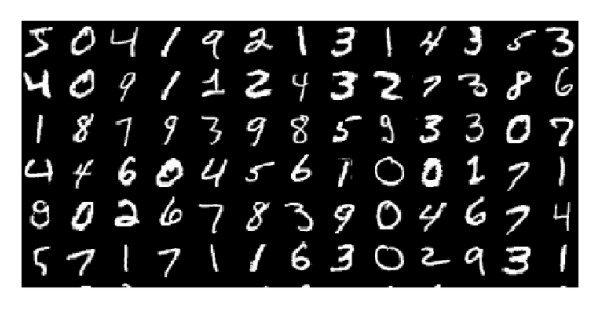
\includegraphics[scale=2.0]{pictures/MNIST.png}
	\caption{Part of samples of MNIST hand-written digit image database\cite{MNISTPIC}.}
	\label{fig:1}
\end{figure}

To fit our model design, we need a pair of data sets with some correlations in between. Our strategy is to cut each image (784 pixels) to upper and lower parts with equal sizes ($28 \times 14$), as shown in Figure 4.2. \\
The upper parts of the images are $x$, and the lower parts of the images are $y$. In this circumstance, $x$ and $y$ are correlated because their features are potentially predictable from one to another. (A human reader will somehow be able to imagine what the other part of a hand-writing 7 or 4 or other digits looks like by looking at one part)\\
Note that given the labels provided by MNIST data indicating which number each image refers to, we group the images by their labels so that each group contains images corresponding to only one digit. We test our model for each group separately. In this case, there will be a greater correlation between two parts of an image because the patterns for a single digit are close even though they come from different writings.
\begin{figure}[H]
	\centering
	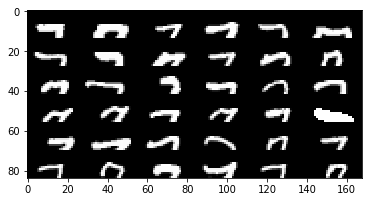
\includegraphics[scale=0.8]{pictures/MNIST_up.png}
	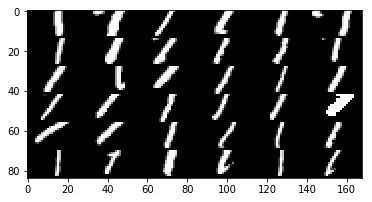
\includegraphics[scale=0.8]{pictures/MNIST_down.png}
	\caption{36 examples of upper and lower parts of digit 7 images.}
	\label{fig:2}
\end{figure}
Based on experimental results, we set the dimension $k=10$ for Principal Component Analysis because the first 10 principal components explain more than 90\% variance of the original image data.

\section{Implementation Detail}
\subsection{TensorFlow}
TensorFlow\cite{TF, TF2} is an open source software library for numerical computation using data flow graphs, a machine learning system that operates at large scale and in heterogeneous environments. Nodes in the graph represent mathematical operations, while the graph edges represent the multidimensional data arrays (tensors) communicated between them. In TensorFlow, developers have the options of deploying computations to one or more CPUs or GPUs in a desktop, server, or mobile device with a single API. TensorFlow was originally developed by researchers and engineers working on the Google Brain Team within Google's Machine Intelligence research organization for the purposes of conducting machine learning and deep neural networks research, but recently this system becomes open to all developers around the world and broadens its range to a wider variety of domains. This architecture gives flexibility to the application developer: whereas in previous “parameter server” designs the management of the shared state is built into the system, TensorFlow enables developers to experiment with novel optimizations and training algorithms. \\
\begin{figure}[H]
	\centering
	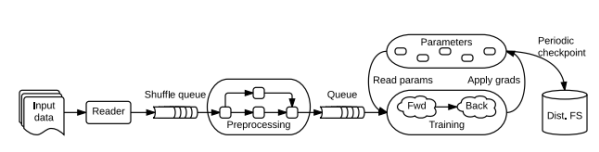
\includegraphics[scale=1.0]{pictures/tensorflow.png}
	\caption{A schematic TensorFlow dataflow graph for a training pipeline, containing subgraphs for reading input data, preprocessing, training, and checkpointing state\cite{TFPIC}.}
	\label{fig:3}
\end{figure}
Based on its great flexibility and programming efficiency, our models are implemented on TensorFlow. 

\subsection{Gradient Descent Optimization}
Gradient descent optimization\cite{GDO} is one of the most popular algorithms to perform optimization and by far the most common way to optimize artificial neural networks. In chapter 3, we mentioned a kernel function optimization training $\kappa$ (3.15), canonical variable to principal component mappings $\gamma$ (3.1) and the encoders $\mathcal{E}$ (3.4). These training processes are implemented by the tool TensorFlow. Here we briefly introduce one of the variants of gradient descent, batch gradient descent, which is applied by TensorFlow class \textit{tf.train.GradientDescentOptimizer}\cite{TFGDO}, to help explain our training algorithm. In code, batch gradient descent looks something like this:
\begin{equation}
\begin{split}
&for\ i\ in\ range ( \#\ epochs ): \\
&\qquad params\_grad = evaluate\_gradient ( cost\_function , data , params ) \\
&\qquad params = params - learning\_rate * params\_grad
\end{split}
\end{equation}
For example, for the following optimization $\phi$ with parameters $W$ and $b$,
\begin{equation}
\begin{split}
&h=f(Wx +b)\\
&cost=\norm{x-x'}_2\\
&\phi=\operatorname*{argmin}_{W,b}cost
\end{split}
\end{equation}
In each step (epoch) $i$, batch gradient descent computes the gradient of the cost function with respect to the parameters for the entire training dataset:
\begin{equation}
\begin{split}
&G({W_i})=\ \dfrac{\partial\ cost}{\partial\ h}\ \dfrac{\partial\ h}{\partial f(W_i)}\ \dfrac{\partial f(W_i)}{dW_i} \\
&G({b_i}) =\ \dfrac{\partial\ cost}{\partial\ h}\ \dfrac{\partial\ h}{\partial f(b_i)}\ \dfrac{\partial f(b_i)}{db_i} \\
&W_{i+1}=W_i - \alpha G(W_i) \\
&b_{i+1}=b_i - \alpha G(b_i)
\end{split}
\end{equation}
where $\alpha$ refers to learning rate and $G()$ refers to the gradient of a parameter. In TensorFlow implementation, we use a one-line code
\begin{center}
	optimizer = tf.train.GradientDescentOptimizer(learning\_rate).minimize(cost)
\end{center}
By this class, we only need to define the learning rate and cost function for a training process. We set the learning rate to 0.01 for all three training processes and the cost functions are described in the previous chapter.

\subsection{Training Parameters}
We set the below training parameters for all training processes in the three model:\\
\textit{hidden layer number = 100, \\
	learning rate = 0.01, \\
	training epochs = 2000, \\
	batch size = 100}\\
From earlier experiments, we found these parameters would ensure that all the steps can be well trained. For a fair comparison, we keep these parameters consistent all the time.

\section{Evaluation Metrics}
To evaluate the reconstruction results, we specify multiple metrics. For image data, for example, the most direct way to check reconstruction performance is to convert the output data back to original canvas size and print the image with reshaped data. Then we can evaluate the reconstruction visually by comparing the reconstruction image with original image. Usually, this is a very effective approach. However, it is not guaranteed that human eyes are able to identify all trivial differences between two images, and it is hard to claim which model works better if two models output similar reconstruction images, or demonstrate visually indistinguishable levels of performance. Thus it is necessary to introduce some quantitative measures. \\
Our purpose here is to compare the reconstructed image data and original image data by quantifying the error, the distance or the similarity between them. This is equivalent to the Image Similarity Analysis\cite{PCC, CC, ISA}. We apply 5 different metrics: $L^2$-norm\cite{NORM}, Pearson Correlation score\cite{PCC}, cross-correlation\cite{CC}, Bhattacharyya distance\cite{ISA} and Fast Fourier Transform (FFT) rank\cite{ISA}.

\subsection{$L^2$-Norm}
For real vectors $x=[x_1,x_2,...x_n]$, $L^2$-Norm\cite{NORM} is given by
\begin{equation}
\norm{x}_2=\sqrt{\sum _{i=1}^{n}x_i^2}
\end{equation}
The $L^2$-Norm is also known as the Euclidean norm because it measures the distance in Euclidean space. For output data vector $x'$ and $y'$, we can measure their reconstruction error by calculating $L^2$-Norm of $x-x'$ and $y-y'$ respectively.
\begin{equation}
\begin{split}
&\norm{x-x'}_2=\sqrt{\sum _{i=1}^{n}(x_i-x'_i)^2} \\
&\norm{y-y'}_2=\sqrt{\sum _{i=1}^{n}(y_i-y'_i)^2}
\end{split}
\end{equation}
Note that $L^2$-Norm works for data as vectors. After reshaping the data to matrix form, the measure turns to Frobenius norm\cite{NORM}. But the result will not change.

\subsection{Pearson Correlation Score}
Pearson Correlation Coefficient\cite{PCC, PCC2} is a measure of the linear correlation between two variables $x$ and $y$. It has a value between -1 and +1, where 1 indicates total positive linear correlation, 0 is no linear correlation, and −1 is total negative linear correlation. Accordingly, Pearson Correlation score measures how highly correlated are two variables. A score of 1 indicates that the data objects are perfectly correlated but in this case, a score of -1 means that the data objects are not correlated. In other words, the Pearson Correlation score quantifies how well two data objects fit a line. \\
In essence, the Pearson Correlation score finds the ratio between the covariance and the standard deviation of both objects. In our case, we calculate the Pearson Correlation score between $x$ and $x'$, $y$ and $y'$ as the following:
\begin{equation}
\begin{split}
&Pearson(x,x')= \dfrac{\sum xx'-\dfrac{\sum x \sum x'}{n}}{\sqrt{(\sum x^2-\dfrac{(\sum x)^2}{n})(\sum x'^2-\dfrac{(\sum x')^2}{n})}}\\
&Pearson(y,y')= \dfrac{\sum yy'-\dfrac{\sum y \sum y'}{n}}{\sqrt{(\sum y^2-\dfrac{(\sum y)^2}{n})(\sum y'^2-\dfrac{(\sum y')^2}{n})}}
\end{split}
\end{equation}
Since the model generates data in the same scale with input data, a larger Pearson Correlation score here refers to greater similarity, thus better reconstruction result.

\subsection{Cross-correlation}
In signal processing, cross-correlation\cite{CC} is a measure of similarity of two series as a function of the displacement of one relative to the other. This measure has been used in medical image registration. For 1-dimensional data, this approach is essentially same as Pearson correlation coefficient score method:
\begin{equation}
\begin{split}
&CC(x,x')=\dfrac{\sum_{i=1}^{n} (x_i-\overline{x})(x'_i-\overline{x'})}{n \sqrt{var(x)var(x')}}\\
&CC(y,y')=\dfrac{\sum_{i=1}^{n} (y_i-\overline{y})(y'_i-\overline{y'})}{n \sqrt{var(y)var(y')}}
\end{split}
\end{equation}
However, for 2-dimensional data, this measure has one advantage: it takes care of the data shifting just like cross-correlation method takes care of the time-delay between signals in signal processing. In our case, let $c2d()$ refers to 2-dimensional cross-correlation computation, for the reshaping data $x,y,x',y' \in \mathbb{R}^{m\times n}$,
\begin{equation}
\begin{split}
&CC2d_x = c2d(\dfrac{x-\overline{x}}{\sqrt{var(x)}},\dfrac{x'-\overline{x'}}{\sqrt{var(x')}})/(m\cdot n) \\
&CC2d_y = c2d(\dfrac{y-\overline{y}}{\sqrt{var(y)}},\dfrac{y'-\overline{y'}}{\sqrt{var(y')}})/(m\cdot n)
\end{split}
\end{equation}
Here $CC2d_x$ and $CC2d_y$ are two arrays containing cross-correlation coefficients (range -1 to 1) in different phases. We select the maximum values of them to represent the similarity between $x$ and $x'$ and between $y$ and $y'$ respectively.

\subsection{Bhattacharyya Distance}
In statistics, the Bhattacharyya distance\cite{BD,BD2,ISA} measures the similarity of two discrete or continuous probability distributions. In image processing, this measure can be used to determine the relative closeness of the two samples being considered. In our case\cite{ISA},
\begin{equation}
\begin{split}
&d(x,x')=\sqrt{1-\dfrac{1}{\sqrt{\overline{xx'}n^2}}\sum_{i=1}^{n} \sqrt{x_{i}x'_{i}}}\\
&d(y,y')=\sqrt{1-\dfrac{1}{\sqrt{\overline{yy'}n^2}}\sum_{i=1}^{n} \sqrt{y_{i}y'_{i}}}
\end{split}
\end{equation}
A zero Bhattacharyya distance means that two data are exactly the same. Larger Bhattacharyya distance refers to greater gap or difference between them.

\subsection{FFT Rank}
Fourier transform\cite{FT} is an important image processing tool which is used to transform an image from spatial domain into frequency domain. A Fast Fourier transform (FFT)\cite{FFT} reduces the complexity of Fourier transform from $N^2$ to $NlogN$. This major improvement of computational makes FFT practically possible in many applications. FFT is an algorithm that samples a signal (or signal-like data) over a period of time (or space) and transforms it into its frequency domain. In the frequency domain, each point represents a particular frequency contained in the spatial domain. The points in frequency domain have both real and imaginary parts, which represent magnitude and phase respectively. In our evaluation of reconstruction, we use only the real part (magnitude) of the FFT results, as it contains most of the information of original data in spatial domain. \\
In our case, we use the following rank formula as our metric for comparison. Here $x,y,x',y'$ refer to intensity values of data (data in spatial domain), and $\overline F_x,\overline F_y,\overline F_{x'},\overline F_{y'}$ represent the average frequency values of them (in frequency domain)\cite{ISA}.
\begin{equation}
\begin{split}
&rank(x,x')=real(\dfrac{(\sum_{i=1}^{n} x_{i}x'_{i}-n\overline F_{x} \overline F_{x'})^2}{(\sum_{i=1}^{n} |x_i|^2-n\overline F_{x}^2)(\sum_{i=1}^{n} |x'_i|^2-n\overline F_{x'}^2)}) \\
&rank(y,y')=real(\dfrac{(\sum_{i=1}^{n} y_{i}y'_{i}-n\overline F_{y} \overline F_{y'})^2}{(\sum_{i=1}^{n} |y_i|^2-n\overline F_{y}^2)(\sum_{i=1}^{n} |y'_i|^2-n\overline F_{y'}^2)})
\end{split}
\end{equation}
A rank ranges from -1 to 1, where 1 is obtained if two datasets are exactly the same and -1 if they are fully independent from each other. The higher the rank, the more similarity shared by the two datasets.

\section{Reconstruction Images}
\subsection{Simple ANNs Reconstruction}
Our initial trial for reconstruction is running a pair of ANNs on the MNIST data sets. This is a simulation of the autoencoders. The neural networks, with one data set as input, are trained to minimize the difference between reconstructed data and the other data set. Consequently, the model builds maps between two correlated data sets.  
\begin{figure}[H]
	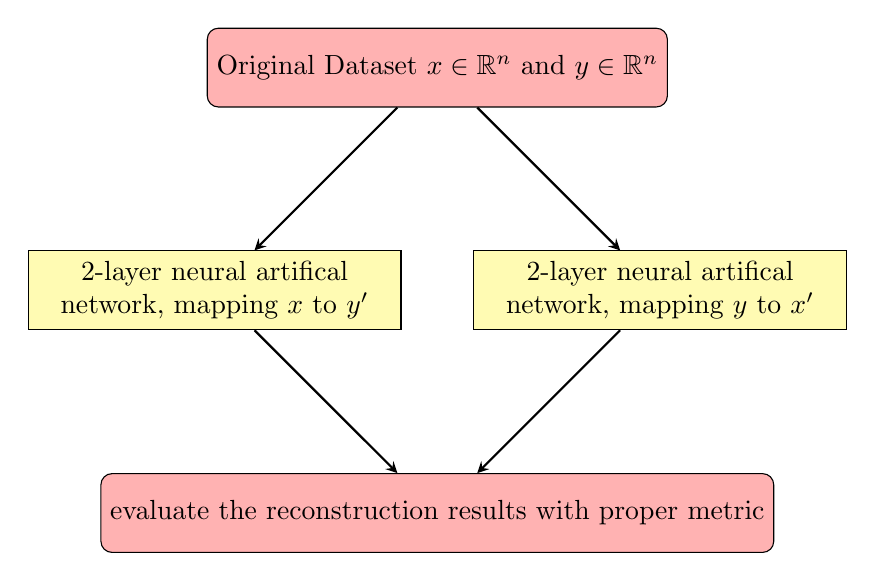
\begin{tikzpicture}[node distance=4cm]
	
	\node (p1) [startstop] {Original Dataset $x\in \mathbb{R}^{n}$ and $y\in \mathbb{R}^{n}$};
	\node (p3) [process, below left of = p1] {2-layer neural artifical network, mapping $x$ to $y'$};
	\node (p4) [process, below right of = p1] {2-layer neural artifical network, mapping $y$ to $x'$};
	
	\draw [arrow] (p1) -- (p3);
	\draw [arrow] (p1) -- (p4);
	
	\node (p5) [startstop, below right of = p3] {evaluate the reconstruction results with proper metric};
	
	\draw [arrow] (p3) -- (p5);
	\draw [arrow] (p4) -- (p5);
	
	\end{tikzpicture}
	\centering
	\caption{Flow chart of the simple paired ANNs. We initially design this model to work like ``paired autoencoders".}
	\label{fig:4}
\end{figure}
The two ANNs above work independently. Each contains a simple two-layer ANN mapping $x$ to $y$ and $y$ to $x$ respectively. All layers follow the classical activation function \(h=\sigma(Wx+b)\). Below are some examples of the reconstruction pictures (we randomly select 6 hand-written images for each digit. The left part of a picture is the original digit image and the right part is the reconstructed image). Although the ANNs reconstruct most of the patterns for these images, it is notable that there are usually some abnormal white pixels in black background. And the positions of these pixels are exactly the same in the samples of each digit. The results indicate that the ANNs learn and ``memorize" a map between the two datasets $x$ and $y$ containing these flaws. This mapping memory prevents the ANNs from perfect reconstruction. We call this issue ``black-to-white" mapping errors. It is an interesting and meaningful theoretical question to explore\cite{DLRG}, but here we are not going to explore it.
\begin{figure}[H]
	\centering
	\subfloat[1 upper]{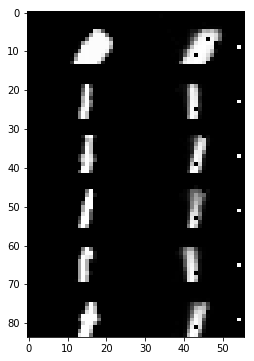
\includegraphics[scale=0.3]{pictures/ANN_1_up.png}} 
	\subfloat[1 lower]{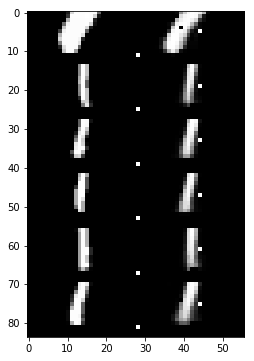
\includegraphics[scale=0.3]{pictures/ANN_1_down.png}}
	\subfloat[7 upper]{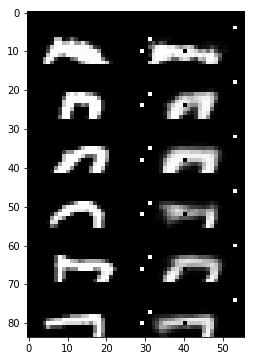
\includegraphics[scale=0.3]{pictures/ANN_7_up.png}}
	\subfloat[7 lower]{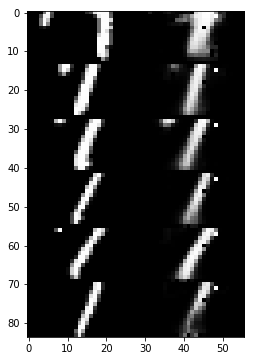
\includegraphics[scale=0.3]{pictures/ANN_7_down.png}} 
	\caption{ANNs Reconstruction of digit 1 and 7}
	\label{fig:5}
\end{figure}

\subsection{NCE, CE and KCE Reconstruction}
\begin{tabular}{m{0.7cm}m{2.4cm}m{2.4cm}m{2.4cm}m{2.4cm}m{2.4cm}m{2.4cm}}
	\toprule
	Digit & KCE Upper & KCE Lower & CE Upper & CE Lower & NCE Upper & NCE Lower\\
	\midrule
	0 & 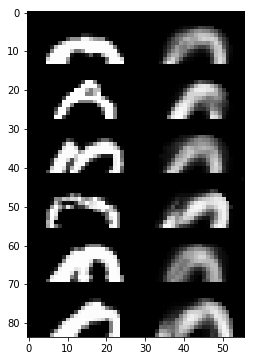
\includegraphics[scale=0.3]{pictures/KE_0_up.png} & 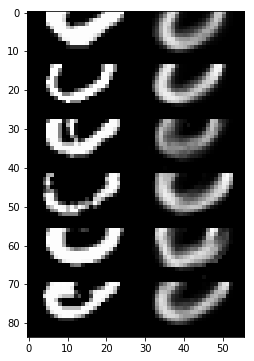
\includegraphics[scale=0.3]{pictures/KE_0_down.png} &
	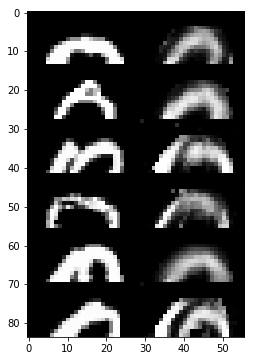
\includegraphics[scale=0.3]{pictures/M1_0_up.png} & 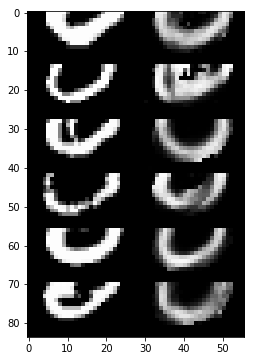
\includegraphics[scale=0.3]{pictures/M1_0_down.png} &
	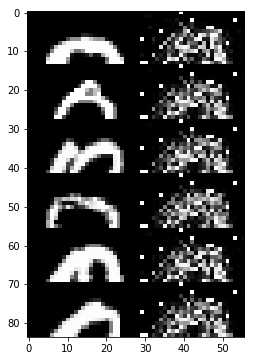
\includegraphics[scale=0.3]{pictures/M2_0_up.png} & 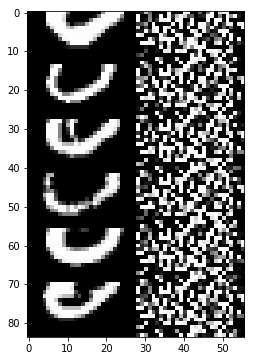
\includegraphics[scale=0.3]{pictures/M2_0_down.png}\\
	1 & 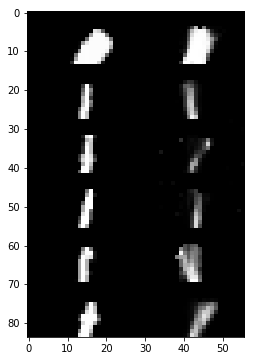
\includegraphics[scale=0.3]{pictures/KE_1_up.png} & 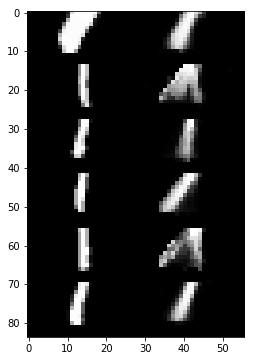
\includegraphics[scale=0.3]{pictures/KE_1_down.png} &
	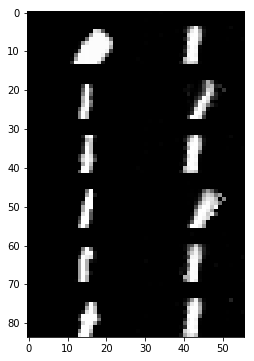
\includegraphics[scale=0.3]{pictures/M1_1_up.png} & 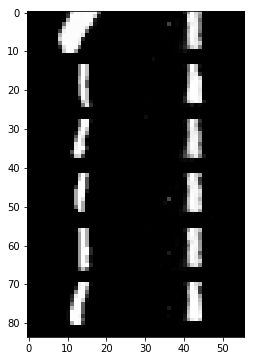
\includegraphics[scale=0.3]{pictures/M1_1_down.png} &
	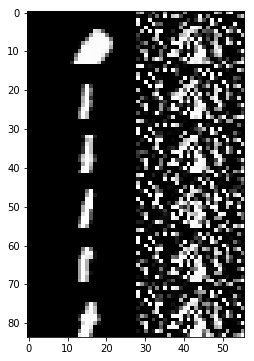
\includegraphics[scale=0.3]{pictures/M2_1_up.png} & 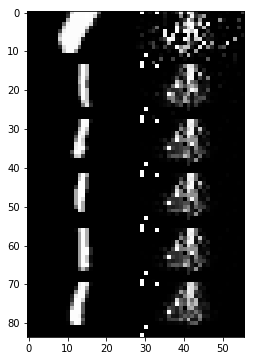
\includegraphics[scale=0.3]{pictures/M2_1_down.png}\\
	2 & 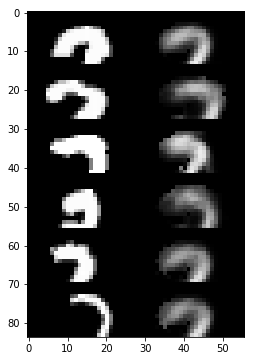
\includegraphics[scale=0.3]{pictures/KE_2_up.png} & 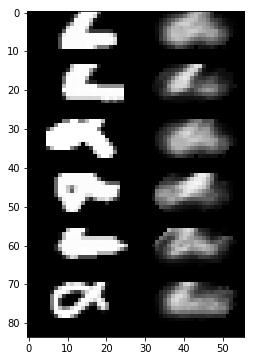
\includegraphics[scale=0.3]{pictures/KE_2_down.png} &
	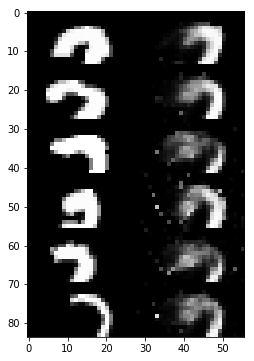
\includegraphics[scale=0.3]{pictures/M1_2_up.png} & 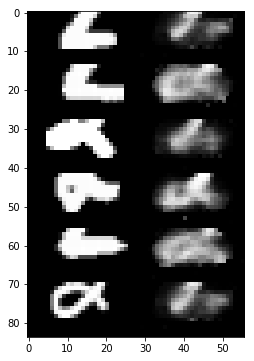
\includegraphics[scale=0.3]{pictures/M1_2_down.png} &
	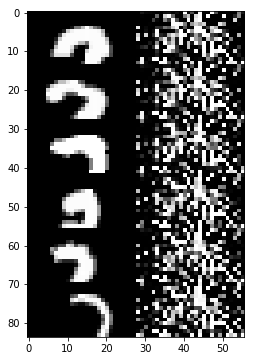
\includegraphics[scale=0.3]{pictures/M2_2_up.png} & 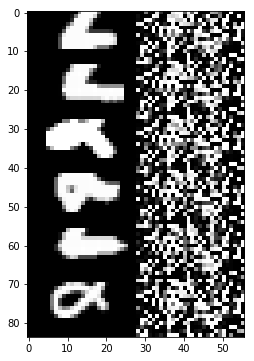
\includegraphics[scale=0.3]{pictures/M2_2_down.png}\\
	3 & 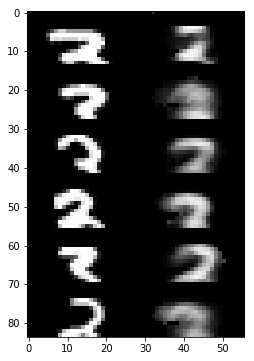
\includegraphics[scale=0.3]{pictures/KE_3_up.png} & 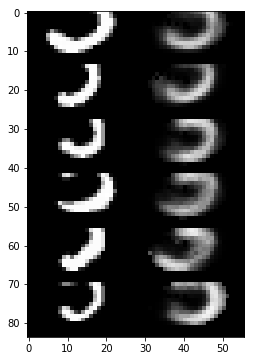
\includegraphics[scale=0.3]{pictures/KE_3_down.png} &
	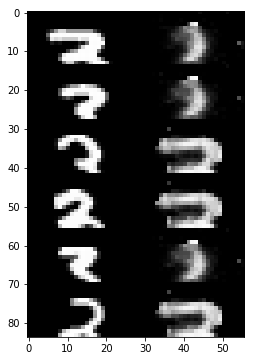
\includegraphics[scale=0.3]{pictures/M1_3_up.png} & 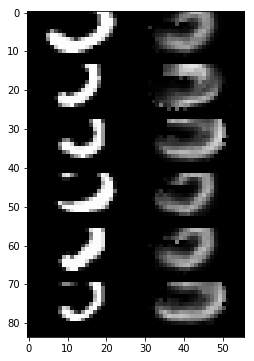
\includegraphics[scale=0.3]{pictures/M1_3_down.png} &
	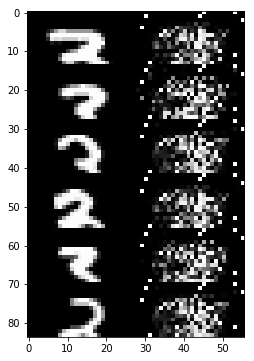
\includegraphics[scale=0.3]{pictures/M2_3_up.png} & 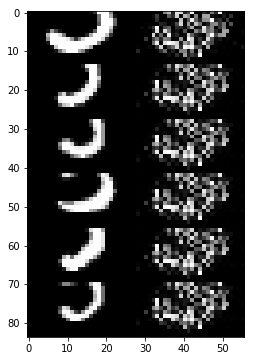
\includegraphics[scale=0.3]{pictures/M2_3_down.png}\\
	4 & 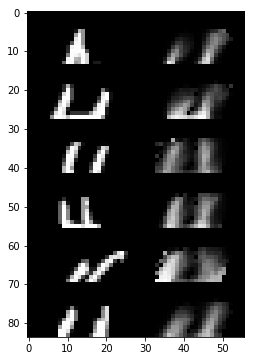
\includegraphics[scale=0.3]{pictures/KE_4_up.png} & 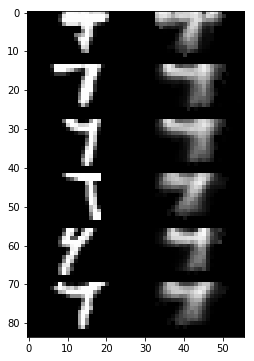
\includegraphics[scale=0.3]{pictures/KE_4_down.png} &
	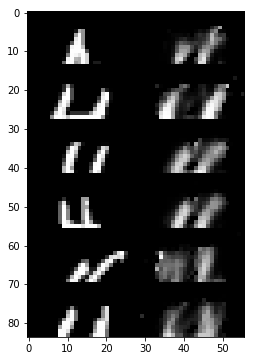
\includegraphics[scale=0.3]{pictures/M1_4_up.png} & 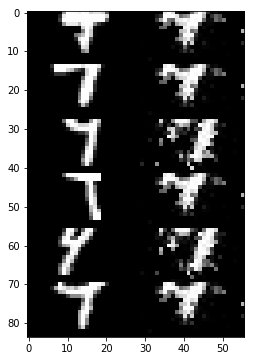
\includegraphics[scale=0.3]{pictures/M1_4_down.png} &
	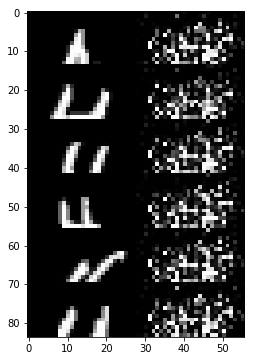
\includegraphics[scale=0.3]{pictures/M2_4_up.png} & 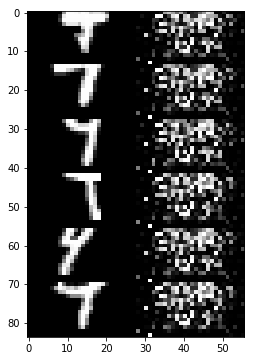
\includegraphics[scale=0.3]{pictures/M2_4_down.png}\\
	%\bottomrule
\end{tabular}

\begin{tabular}{m{0.7cm}m{2.4cm}m{2.4cm}m{2.4cm}m{2.4cm}m{2.4cm}m{2.4cm}}
	%\toprule
	%Digit & KCE Upper & KCE Lower & CE Upper & CE Lower & NCE Upper & NCE Lower\\
	%\midrule
	5 & 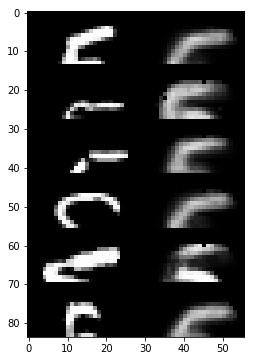
\includegraphics[scale=0.3]{pictures/KE_5_up.png} & 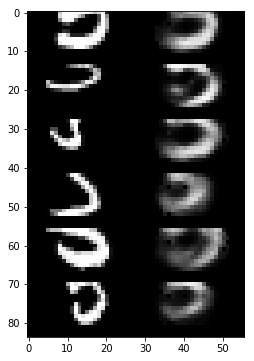
\includegraphics[scale=0.3]{pictures/KE_5_down.png} &
	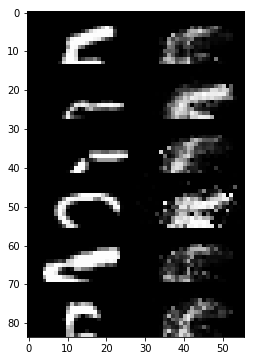
\includegraphics[scale=0.3]{pictures/M1_5_up.png} & 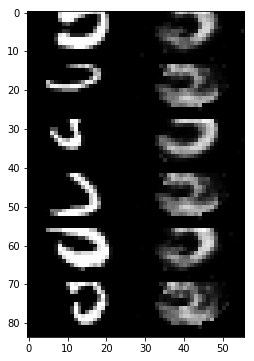
\includegraphics[scale=0.3]{pictures/M1_5_down.png} &
	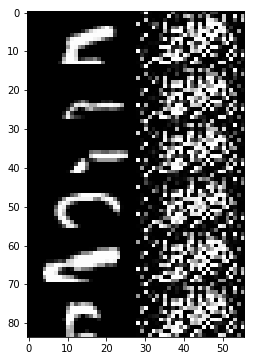
\includegraphics[scale=0.3]{pictures/M2_5_up.png} & 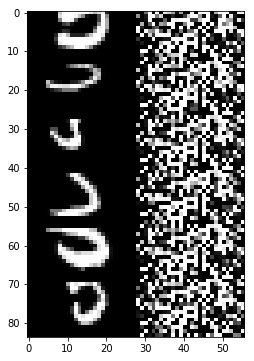
\includegraphics[scale=0.3]{pictures/M2_5_down.png}\\
	6 & 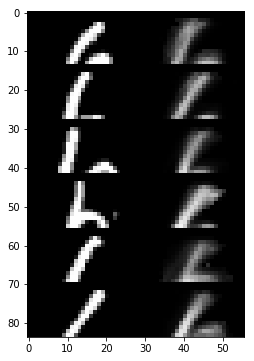
\includegraphics[scale=0.3]{pictures/KE_6_up.png} & 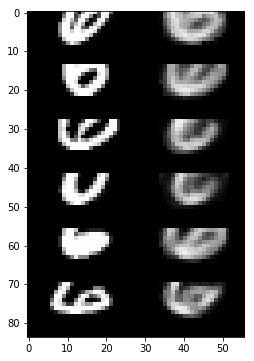
\includegraphics[scale=0.3]{pictures/KE_6_down.png} &
	\includegraphics[scale=0.3]{pictures/M1_6_up.png} & \includegraphics[scale=0.3]{pictures/M1_6_down.png} &
	\includegraphics[scale=0.3]{pictures/M2_6_up.png} & \includegraphics[scale=0.3]{pictures/M2_6_down.png}\\
	7 & \includegraphics[scale=0.3]{pictures/KE_7_up.png} & \includegraphics[scale=0.3]{pictures/KE_7_down.png} &
	\includegraphics[scale=0.3]{pictures/M1_7_up.png} & \includegraphics[scale=0.3]{pictures/M1_7_down.png} &
	\includegraphics[scale=0.3]{pictures/M2_7_up.png} & \includegraphics[scale=0.3]{pictures/M2_7_down.png}\\
	8 & \includegraphics[scale=0.3]{pictures/KE_8_up.png} & \includegraphics[scale=0.3]{pictures/KE_8_down.png} &
	\includegraphics[scale=0.3]{pictures/M1_8_up.png} & \includegraphics[scale=0.3]{pictures/M1_8_down.png} &
	\includegraphics[scale=0.3]{pictures/M2_8_up.png} & \includegraphics[scale=0.3]{pictures/M2_8_down.png}\\
	9 & \includegraphics[scale=0.3]{pictures/KE_9_up.png} & \includegraphics[scale=0.3]{pictures/KE_9_down.png} &
	\includegraphics[scale=0.3]{pictures/M1_9_up.png} & \includegraphics[scale=0.3]{pictures/M1_9_down.png} &
	\includegraphics[scale=0.3]{pictures/M2_9_up.png} & \includegraphics[scale=0.3]{pictures/M2_9_down.png}\\
	\bottomrule
\end{tabular}
\\
\\
In the above table, we post all the reconstruction results of testing. In the testing part, we randomly select 6 hand-written images for each digit from test data set and run all three models on these samples. Thus in each picture, we have 6 original half-images on the left and 6 reconstructed half-images on the right. The table contains reconstruction results from KCE, CE and NCE. \\
Note, here we set KCE as the benchmark for comparison. The essential purpose is to demonstrate the effectiveness of KCCA compared with linear CCA and non-CCA in our task. Since the decoder phases are identical within all three models, the reconstruction results can reflect the effective of the encoder phase, more specifically, KCCA, CCA or neither. \\
From the results shown in the table, we can visually evaluate the performances of the three models. First, contrasting the results of KCE with the results of NCE, it is obvious that KCE generates better reconstruction. This is a convincing clue to claim the effectiveness of KCCA step. With the help of KCCA, the reconstruction images become identifiable and clean. Then we compare KCE with CE, the differences are not as easily observable. The patterns of hand-written digits are generally reconstructed in both models. However, the patterns of some reconstructed images from CE, such as upper part of 5 and lower part of 4 are smashed to pieces while this never occur in KCE reconstruction. To authenticate the difference, we need to take a further step to quantitative metrics. Notably, compared with the images from ANNs reconstruction, we find that KCE solves the ``black-to-white" mapping problem.

\section{Quantitative Comparison}
We use the 5 metrics for Image Similarity Analysis introduced in section 3.3 to quantitatively evaluate the performances of our three models. For each model, we have 6 pairs of reconstructed image data sets for each digit 0-9, thus 120 arrays of data with size 392 ($28 \times 14$), the total pixel number for one half-image. We do the image similarity analysis for KCE, CE and NCE by comparing their reconstructed data with the original data to indicate the similarities between the original images and reconstructed images. For each one of the metric, we calculate the mean of 120 scores/distances/ranks of the three models separately. Then we do T-tests\cite{TTEST} to compare KCE with CE and NCE respectively. We extract p-values indicating the confidence to claim that scores/distances/ranks are different (the smaller the p-value, the more confident to claim this). The statistical analysis results are shown in Table 4.1 and Table 4.2.

\begin{table}[H]
	\centering
	\begin{tabular}{m{5cm}m{3cm}m{3cm}m{3cm}}
		\toprule
		Metric & NCE average & KCE average & p-value \\
		\midrule
		2-norm & 8.3188 & \textcolor{cyan}{4.93307} & \textcolor{red}{1.07055e-38} \\
		Pearson Coefficient & 0.295733 & \textcolor{cyan}{0.607328} & \textcolor{red}{2.36711e-28} \\
		cross correlation & 0.344092 & \textcolor{cyan}{0.711152} & \textcolor{red}{1.04487e-58} \\
		Bhattacharyya distance & 0.693693 & \textcolor{cyan}{0.507269} & \textcolor{red}{5.28491e-29} \\
		FFT & 0.204558 & \textcolor{cyan}{0.489945} & \textcolor{red}{3.99356e-27} \\
		\bottomrule
	\end{tabular}
    \caption{Statistical results between KCE and NCE: the light blue highlights indicate better performance between KCE and NCE while the red highlights indicate p-value less than 0.05. The 5 metrics all demonstrate better performance to KCE with p-values lower than 0.05. we claim that KCE generates better reconstruction results than NCE.}
\end{table}

\begin{table}[H]
	\centering
	\begin{tabular}{m{5cm}m{3cm}m{3cm}m{3cm}}
		\toprule
		Metric & CE average & KCE average & p-value \\
		\midrule
		2-norm & 5.41653 & \textcolor{cyan}{4.94215} & \textcolor{red}{0.00297353} \\
		Pearson Coefficient & 0.550588 & \textcolor{cyan}{0.618759} & \textcolor{red}{0.00663332} \\
		cross correlation & 0.689174 & \textcolor{cyan}{0.712149} & 0.113121 \\
		Bhattacharyya distance & 0.539608 & \textcolor{cyan}{0.505529} & \textcolor{red}{0.0272345} \\
		FFT & 0.42421 & \textcolor{cyan}{0.4972} & \textcolor{red}{0.00352892} \\
		\bottomrule
	\end{tabular}
	\caption{Statistical results between KCE and CE: the light blue highlights indicate better performance between KCE and CE while the red highlights indicate p-value less than 0.05. Since all metrics point to the greater similarity between KCE reconstruction and original data and most p-values are less than the confidence threshold 0.05, we claim that KCE generates better reconstruction results than CE.}
\end{table}


In general, from the statistics provided in the tables, no matter compared with CE or NCE, the average values of all 5 metrics show that KCE has greater performance. Meanwhile, most of (9/10) the p-values are less than 0.05, small enough to support this claim. The results demonstrate that in our reconstruction task, KCE has better performance than the two comparison models. This further proves the effectiveness of KCCA. 

\chapter{Conclusion}
\section{Contribution}
In this research, we propose three models to find complex correlations between two variables and KCE model demonstrates the best performance on a high dimensional image reconstruction task. Given two potentially correlated high-dimensional data sets, KCE successfully builds a map between the two data sets. Thus we can reconstruct one data set by the other and their mutual information. Our research starts with exploration on the limitation of CCA on high dimensional data through several experiments. In addition, with the help of Mercer's theorem and Schoenberg's theorem, we improve CCA by introducing kernel methods that map data to RKHS and improve the coherence calculation. In the processes of mapping canonical variables to the original feature space of another data set, we try both linear and non-linear ANNs and figure out that a linear ANN before PCA reconstruction and a non-linear ANN after PCA reconstruction best fit our demand. Our model solves the ``black-to-white" mapping error problem for gray-scale image reconstruction. Meanwhile, we prove the effectiveness of KCCA in the paired reconstruction task.

\section{Future Work}
We propose three directions for the future work:\\
First, we believe that during the PCA projection, some information of original data gets lost. We will run more experiments to explore the dimensionality trade-off for better reconstruction results.\\
Second, we have observed that our model is able to avoid the ``black-to-white" mapping error problem. It is worth for us to dig out the reason and continue to produce a mathematical proof for this.\\
Third, so far we have only done the experiments on MNIST data. We should explore more samples including face images, item images or even other types of data to justify the effectiveness of our model.

\begin{thebibliography}{}

    \bibitem{KCCA}
	Lai, Pei Ling, and Colin Fyfe. "Kernel and nonlinear canonical correlation analysis." \textit{International Journal of Neural Systems10.05 (2000): 365-377.}

	\bibitem{AE}
	Tan, Chun Chet. Autoencoder neural networks: A performance study based on image reconstruction, recognition and compression. \textit{LAP Lambert Academic Publishing, 2009.}

	\bibitem{AE2}
	aymericdamien, TensorFlow-Examples, (2017), GitHub repository, \textit{https://github.com/aymericdamien/TensorFlow-Examples}

	\bibitem{AE3}
	Baldi, Pierre. "Autoencoders, unsupervised learning, and deep architectures." \textit{Proceedings of ICML Workshop on Unsupervised and Transfer Learning. 2012.}

	\bibitem{ECCA}
	Pezeshki, A., Scharf, L. L., Azimi-Sadjadi, M. R., \& Lundberg, M. (2004, November). Empirical canonical correlation analysis in subspaces. \textit{In Signals, Systems and Computers, 2004. Conference Record of the Thirty-Eighth Asilomar Conference on (Vol. 1, pp. 994-997). IEEE.}

	\bibitem{PCA}
	Wold, Svante, Kim Esbensen, and Paul Geladi. "Principal component analysis." \textit{Chemometrics and intelligent laboratory systems 2.1-3 (1987): 37-52.}

	\bibitem{PCA2}
	Pearson, K. (1901). "On Lines and Planes of Closest Fit to Systems of Points in Space". \textit{Philosophical Magazine. 2 (11): 559–572.}

	\bibitem{REPCA}
	amoeba (https://stats.stackexchange.com/users/28666/amoeba), How to reverse PCA and reconstruct original variables from several principal components?, URL (version: 2016-08-12): \textit{https://stats.stackexchange.com/q/229092}

	\bibitem{AUKM}
	Autoencoder Using Kernel Methods
	\textit{http://technodocbox.com/3D\_Graphics/66255915-Autoencoder-using-kernel-method.html}

	\bibitem{RKHS}
	Gretton, Arthur. "Introduction to rkhs, and some simple kernel algorithms."
	\textit{Adv. Top. Mach. Learn. Lecture Conducted from University College London (2013): 16.}

	\bibitem{GM}
	Gram matrix. Encyclopedia of Mathematics. \\
	URL:\textit{http://www.encyclopediaofmath.org/index.php?title=Gram\_matrix\&oldid=35177}

	\bibitem{SM}
	Weisstein, Eric W. "Singular Matrix." From MathWorld--A Wolfram Web Resource. \textit{http://mathworld.wolfram.com/SingularMatrix.html}

	\bibitem{CCA}
	Härdle, Wolfgang; Simar, Léopold (2007). "Canonical Correlation Analysis". \textit{Applied Multivariate Statistical Analysis. pp. 321–330. doi:10.1007/978-3-540-72244-1\_14. ISBN 978-3-540-72243-4.}

	\bibitem{TF}
	Abadi, Martín, et al. "TensorFlow: A System for Large-Scale Machine Learning."
	\textit{OSDI. Vol. 16. 2016.}

	\bibitem{TF2}
	"Credits". \textit{TensorFlow.org}. Retrieved November 10, 2015.

	\bibitem{TF3}
	"TensorFlow Release". Retrieved February 28, 2018.

	\bibitem{STAT}
	James, Gareth, et al. An introduction to statistical learning.
	\textit{Vol. 112. New York: springer, 2013.}

	\bibitem{PR}
	Theodoridis, Sergios (2008). Pattern Recognition. \textit{Elsevier B.V. p. 203. ISBN 9780080949123.}

	\bibitem{PD}
	Hein, Matthias, and Olivier Bousquet. "Hilbertian metrics and positive definite kernels on probability measures."
	\textit{AISTATS. 2005.}

	\bibitem{MT}
	Mercer, J. (1909), "Functions of positive and negative type and their connection with the theory of integral equations", \textit{Philosophical Transactions of the Royal Society A, 209 (441–458): 415–446}

	\bibitem{CMF}
    Miller, Kenneth S., and Stefan G. Samko. "Completely monotonic functions." \textit{Integral Transforms and Special Functions 12.4 (2001): 389-402.}

	\bibitem{Schoenberg}
	Schoenberg Ann. of Math. textit{39 (1938), 811-841)}

	\bibitem{DL}
	Deng, Li, and Dong Yu. "Deep learning: methods and applications." \textit{Foundations and Trends in Signal Processing 7.3–4 (2014): 197-387.}

	\bibitem{NN}
	Schmidhuber, Jürgen. "Deep learning in neural networks: An overview." \textit{Neural networks 61 (2015): 85-117.}

	\bibitem{NN2}
	Wang, Sun-Chong. "Artificial neural network." \textit{Interdisciplinary computing in java programming. Springer, Boston, MA, 2003. 81-100.}

	\bibitem{MC}
	Maxwell, Scott E., Harold D. Delaney, and Ken Kelley. Designing experiments and analyzing data: A model comparison perspective. \textit{Routledge, 2017.}

	\bibitem{KPCA}
	Schölkopf, Bernhard, Alexander Smola, and Klaus-Robert Müller. "Nonlinear component analysis as a kernel eigenvalue problem." \textit{Neural computation 10.5 (1998): 1299-1319.}

	\bibitem{TFGDO}
	Tensorflow Class GradientDescentOptimizer, \\
    URL:\textit{https://www.tensorflow.org/api\_docs/python/tf/train/GradientDescentOptimizer}

	\bibitem{GDO}
	Ruder, Sebastian. "An overview of gradient descent optimization algorithms." \textit{arXiv preprint arXiv:1609.04747 (2016).}

	\bibitem{PCC}
	Segaran, Toby. Programming Collective Intelligence: Building Smart Web 2.0 Applications. \textit{Sebastopol, CA: O'Reilly Media, 2007.}

	\bibitem{ISA}
	Narayanan, Siddharth, and P. K. Thirivikraman. "IMAGE SIMILARITY USING FOURIER TRANSFORM." \textit{Journal Impact Factor 6.2 (2015): 29-37.}

	\bibitem{NORM}
	Gradshteyn, I. S. and Ryzhik, I. M. Tables of Integrals, Series, and Products, 6th ed. \textit{San Diego, CA: Academic Press, pp. 1114-1125, 2000.}

    \bibitem{PCC2}
	"SPSS Tutorials: Pearson Correlation". Retrieved 2017-05-14.

	\bibitem{CC}
	Avants, Brian B., et al. "Symmetric diffeomorphic image registration with cross-correlation: evaluating automated labeling of elderly and neurodegenerative brain." \textit{Medical image analysis 12.1 (2008): 26-41.}

	\bibitem{BD}
	Bhattacharyya, A. (1943). "On a measure of divergence between two statistical populations defined by their probability distributions". \textit{Bulletin of the Calcutta Mathematical Society.}

	\bibitem{BD2}
	Guorong, Xuan, Chai Peiqi, and Wu Minhui. "Bhattacharyya distance feature selection." \textit{Pattern Recognition, 1996., Proceedings of the 13th International Conference on. Vol. 2. IEEE, 1996.}

	\bibitem{FT}
	Bracewell, Ronald Newbold, and Ronald N. Bracewell. The Fourier transform and its applications. \textit{Vol. 31999. New York: McGraw-Hill, 1986.}

	\bibitem{FFT}
	Bergland, G. D. "A Guided Tour of the Fast Fourier Transform." \textit{IEEE Spectrum 6, 41-52, July 1969.}

	\bibitem{MNIST}
	Tensorflow Digit Dataset
	\textit{https://www.tensorflow.org/get\_started/mnist/beginners}

	\bibitem{DLRG}
	Zhang, Chiyuan, et al. "Understanding deep learning requires rethinking generalization." \textit{arXiv preprint arXiv:1611.03530(2016).}

	\bibitem{TTEST}
	Devore, Jay, Nicholas Farnum, and Jimmy Doi. Applied statistics for engineers and scientists. \textit{Nelson Education, 2013.}

	\bibitem{KPIC}
	Picture resource by Bioinformatics Lab, ICGEB, New Delhi,
	\textit{http://bioinfo.icgeb.res.in/lipocalinpred/algorithm.html}

	\bibitem{NNPIC}
	Picture resource by Glosser.ca - Own work, Derivative of File:Artificial neural network.svg, CC BY-SA 3.0, \textit{https://commons.wikimedia.org/w/index.php?curid=24913461}

	\bibitem{SIGPIC}
	Picture resource by Qef (talk) - Created from scratch with gnuplot, Public Domain, \textit{https://commons.wikimedia.org/w/index.php?curid=4310325}

	\bibitem{AEPIC}
	Picture resource by Chervinskii - Own work, CC BY-SA 4.0,  \textit{://commons.wikimedia.org/w/index.php?curid=45555552}

	\bibitem{TFPIC}
	Picture resource by Abadi, Martín, et al. "TensorFlow: A System for Large-Scale Machine Learning." \textit{OSDI. Vol. 16. 2016.}

	\bibitem{MNISTPIC}
	Picture resource by Cheng, Chunling, et al. "A multilayer improved RBM network based image compression method in wireless sensor networks." \textit{International Journal of Distributed Sensor Networks 12.3 (2016): 1851829.}


\end{thebibliography}
\end{document}
